\documentclass[11pt]{article}
%
%%%%%%%%%%%%%%%%%%%%%%%%%%%%%%%%%%%%
%% Common preamble
%%%%%%%%%%%%%%%%%%%%%%%%%%%%%%%%%%%%
% PAGE
\newcommand{\tuta}{\emph{T.~absoluta}}
\newcommand{\infest}{\rho}
\newcommand{\totinf}{\rho_{\mathrm{T}}}
\newcommand{\suitable}{\epsilon}
%% \usepackage{fullpage} % uncomment this when changing to jour/conf style
%% % FONTS
%% \usepackage{lmodern} % enhanced version of computer modern
%% \usepackage[T1]{fontenc} % for hyphenated characters and textsc in section title
%% \usepackage{xr}
%% \externaldocument{supplementary}
\usepackage{microtype} % some compression
\usepackage{times}
\usepackage{setspace} % For double line spacing
\doublespacing
\usepackage[left=1in,top=1in,right=1in,bottom=1in]{geometry}
\usepackage[pagewise]{lineno}
\usepackage{marvosym}
\linenumbers
% MATH
\usepackage{amssymb}
\usepackage{mathtools} % contains amsmath which comes with align
\usepackage{amsthm} % newtheorem stuff
\usepackage{bm} % for bold math (use $\boldsymbol{}$)
% COLOR
\usepackage[usenames,dvipsnames]{color}
%%
% REFERENCING
% JM: Below is for affiliations
\usepackage{authblk}
% BIBLIOGRAPHY
\usepackage[square,sort&compress,numbers]{natbib} %sorts bibs when they are collectively cited
\usepackage[colorlinks=true,pdfborder={0 0 0},citecolor=RoyalBlue,linkcolor=black,urlcolor=Magenta]{hyperref}
\usepackage{cleveref} %%% IMPORTANT: cleveref comes before \newtheorem commands
   \crefname{figure}{Figure}{Figures}
   \crefname{table}{Table}{Tables}
   \crefname{theorem}{Theorem}{Theorems}
   \crefname{lemma}{Lemma}{Lemmas}
   \crefname{claim}{Claim}{Claims}
   \crefname{section}{Section}{Sections}
   \crefname{observation}{Observation}{Observations}
   \crefname{note}{Note}{Notes}
%%
% TABLES
\usepackage{multirow}
%% \usepackage{ctable} % provides toprule, bottomrule, midrule
\usepackage{array} % new implementation of tabular & array with lots of enhancements
%%
% FIGURES
\usepackage{graphicx}
\graphicspath{./figs}
\usepackage{grffile} % to set right names of files
%%
% CAPTIONS
\usepackage{caption}
\usepackage{subcaption} % supersedes subfigure & subfloat. try using options
%%
% LISTS
\usepackage{enumitem} %\begin{itemize}[leftmargin=*]
%% inline
\newlist{inline}{enumerate*}{1}
\setlist[inline]{before=\unskip{: }, itemjoin={{; }}, itemjoin*={{; and }}, label={(\roman*)}}
% ALGO
\usepackage[ruled,linesnumbered]{algorithm2e}
%% comments & todo
\newcommand{\reportingCells}{\mathcal{C}_R}
\newcommand{\likelihood}{\mathcal{L}}
\newcommand{\aacomment}[1]{({\color{magenta}AA: #1})}
\newcommand{\mmcomment}[1]{({\color{green}MM: #1})}
\newcommand{\tbcomment}[1]{({\color{blue}TB: #1})}
\newcommand{\mrccomment}[1]{({\color{red}MRC: #1})}
\usepackage[colorinlistoftodos]{todonotes}
\newcommand{\TODO}[1]{\todo[inline,color=red!10,size=\small]{#1}}
%% COMMANDS
\newcommand{\comp}[1]{\overline{#1}}  %{\widetilde{#1}}
\DeclareMathOperator{\Var}{Var}
\DeclareMathOperator{\Cov}{Cov}
\DeclareMathOperator{\bigo}{O}
\DeclareMathOperator{\bigom}{\Omega}
\DeclareMathOperator{\davg}{d_{avg}}
\DeclareMathOperator*{\argmax}{arg\,max}
\DeclareMathOperator*{\argmim}{arg\,min}
% Note: \deg is already defined
\newcommand{\expect}{\mathbb{E}}
%
\newcommand{\ceil}[1]{\left\lceil #1 \right\rceil}
\newcommand{\floor}[1]{\left\lfloor #1 \right\rfloor}
%
\newcommand{\reals}{\mathbb{R}}
\newcommand{\field}{\mathbb{F}}
\newcommand{\integers}{\mathbb{Z}}
%
\newtheorem{theorem}{Theorem}[]{\bfseries}{\itshape} 
\newtheorem{lemma}[theorem]{Lemma}{\bfseries}{\itshape}
\newtheorem{claim}[theorem]{Claim}{\bfseries}{\itshape}
\theoremstyle{definition}
\newtheorem{definition}[theorem]{Definition} % {\bfseries}{\itshape}
\newtheorem{observation}[theorem]{Observation} % {\bfseries}
\newtheorem{condition}[theorem]{Condition} % {\bfseries}{\itshape}
\newtheorem{note}[theorem]{Note} % {\bfseries}{\itshape}
% ROMAN NUMERALS
\makeatletter
\newcommand{\rmnum}[1]{\romannumeral #1}
\newcommand{\Rmnum}[1]{\expandafter\@slowromancap\romannumeral #1@}
\makeatother
%%
% TWO VERSIONS
%% \usepackage{etoolbox}
%% \newtoggle{withappendix}
%% \toggletrue{withappendix} % comment this if you want journal version
%% Usage: iftoggle{withappendix}{}{}
%%
%% math operator
%% \DeclareMathOperator{\sgn}{sgn}
% CODEBOX
%% \usepackage[framemethod=tikz]{mdframed}
%% \newmdenv[linecolor=black!10,innerlinewidth=0pt, roundcorner=4pt,innerleftmargin=6pt,
%% font=\ttfamily,innerrightmargin=6pt,innertopmargin=6pt,
%% innerbottommargin=6pt,backgroundcolor=black!10]{codeblock}
%%%%%%%%%%%%%%%%%%%%%%%%%%%%%%%%%%%%
%% preamble ends
%% from now on, draft specific
%%%%%%%%%%%%%%%%%%%%%%%%%%%%%%%%%%%%
%% \RequirePackage[l2tabu, orthodox]{nag}
\makeatletter
\renewcommand\AB@affilsepx{, \protect\Affilfont}
\makeatother

\title{A Multi-pathway Modeling Approach to Assess the Threat of
\emph{Tuta~absoluta} in Southeast~Asia}
\author[1]{Joseph~McNitt}
\author[1]{Young~Yun~Chungbaek}
\author[1]{Henning~Mortveit}
\author[1]{Madhav~Marathe}
\author[2]{Mateus~Ribeiro~de~Campos}
\author[2]{Nicolas~Desneux}
\author[3]{Thierry~Br\'{e}vault}
\author[4]{Rangaswamy Muniappan}
\author[1]{Abhijin~Adiga}
\affil[1]{Biocomplexity Institute of Virginia Tech}
\affil[2]{French National Institute for Agricultural Research}
\affil[3]{CIRAD, BIOPASS}
\affil[4]{Feed the Future Integrated Pest Management Innovation Lab}
\date{}
\setcounter{Maxaffil}{0}
\renewcommand\Affilfont{\itshape\small}

\begin{document}
\maketitle

\begin{abstract}
\emph{Tuta absoluta} is a devastating pest of tomato which has
spread in Europe, Africa, and Asia over the last decade. There is strong
evidence of multiple pathways, both natural and human-assisted, for its
rapid range expansion. We propose a generic data-driven epidemiological
modeling approach to study this complex phenomenon accounting for biology,
seasonal production, trade and demographic information. We apply this model
to study the dynamics of \tuta{} spread in South and Southeast Asia -- a
region at the frontier of its current range. Our objective is to assess the
possible routes of introduction, the role of different pathways in the
spread and predict its spread pattern in the study region.

Our analysis with respect to incidence reports strongly suggests the role
of both natural and human-assisted pathways in the spread of \tuta{}.
Applying the model to the rest of the study region, we predict that within
five years \tuta{} will invade all the major vegetable growing areas of
mainland Southeast Asia if no steps are taken to mitigate the spread. We
also consider alternate scenarios of introduction of the pest to the region
through trade and travel.  
%% Further, we show that monitoring and effective interventions
%% at the market level can reduce the speed of the spread.
\end{abstract}
%%
\section{Introduction}
%%
The world is witnessing a rapid increase in global trade and
travel~\cite{ercsey2012complexity}. Due to this increased global
connectivity, both international and domestic, no region is spared of the
threat from exotic species invasion~\cite{hulme2009trade}.  
climate change and detrimental impact of intensive agriculture on natural
resources are likely to further aggravate the problem. As a result, global food security,
human health and social welfare will be adversely impacted. The South
American Tomato leafminer, or \emph{Tuta absoluta}, is a representative
example of biological invasion that has significantly affected tomato
production worldwide in the last decade.

Indigenous to South America, \tuta{} was accidentally introduced to Spain
in~2006~\cite{desneux2010biological,biondi2017}. Since then, it has rapidly
spread throughout Europe, Africa, Western Asia, the Indian subcontinent,
and parts of Central America~\cite{campos2017western}. In South Asia, the
pest was first reported by India
in~2014~\cite{sridhar2014new,kalleshwaraswamy2015occurrence}.  By
early~2016, it was discovered in the Kathmandu area of
Nepal~\cite{bajracharya2016first}, the northern part of Bangladesh in
May~2016~\cite{hossain2016first}, and then in northeastern
India~\cite{sankarganesh2017}.  The speed of he spread poses a significant time critical
threat to tomato cultivation in Southeast Asia. In order to effectively respond,
one needs to identify possible routes of introduction and likely
spatio-temporal patterns of spread in this region.  With tomato being a
commercially important crop, this invastion has had significant global
impact.  For example, in the Netherlands and Turkey alone, the annual
estimated intervention cost are \EURdig4 and \EURdig167 millions per year,
respectively~\cite{potting2013tuta,oztemiz2014tuta}. Due to extensive
insecticide treatment in Europe, insecticidal resistance has been recently
observed in populations~\cite{guedes2013tomato}. Overall, lack of effective
indigenous predators has made integrated pest management (IPM) a
challenging task.
%%

Since tomato is among the top two traded vegetables in the world (\url{http://www.fao.org}),
it is strongly suspected that trade played a critical role in \tuta{}'s
rapid spread~\cite{campos2017western}. Indeed, on multiple occasions it has
been discovered in packaging stations (\cite{eppo105} for example). It was
observed that the spread pattern in Bulgaria was correlated with prime
trade routes~\cite{karadjova2013tuta}.  The Animal and Plant Health
Inspection Service of the United States Department of Agriculture
(USDA-APHIS) has instituted quarantine regulations for imports from regions
where the pest is present~\cite{USDA2012}. Rapid increase in protected
cultivation methods such as green houses and tunnel farming have allowed it
to overwinter as well as survive the wet season.

Faced with the challenging task of preparing for the invasion of 
pests and pathogens, and responding effectively to mitigate such incursions
should they happen, decision makers are increasingly relying on  computational
models of pest risk maps and spread to aid decision making~\cite{venette2010}.
While models that create pest risk maps (e.g. CLIMEX) are useful to
identify locations which are suitable for long-term establishment, % and cause harmful impact
spread models help specify the spatio-temporal
dynamics of how the pest spreads.  The latter approach is particularly useful in planning
for the possible threat from an invasive
species~\cite{perrings2014merging,barbier2013implementing,paini2010threat,paini2010threat,paini2016global}
through {\it in silico} experiments simulating
hypothetical invasion scenarios. Together, these tools can be used to
address questions such as which locations to monitor, what control measures
to take (areawide IPM practices, trade restrictions, etc.), what is the
impact on the economy and health, and so on.

Although there is a general consensus that vegetable and seedling trade is a
primary driver of \tuta{} spread, previous modeling efforts have
exclusively focused on ecological aspects. Two
studies~\cite{desneux2010biological,tonnang2015identification} provide risk
maps using CLIMEX and take additional factors into account.
Guimapi~et~al.~\cite{guimapi2016modeling} used a
cellular automata approach to capture the global spread of the pest by
factoring in temporal variations and spatial distribution of vegetation,
temperature, and tomato production. In recent years, the role of
human-mediated dispersal is increasingly accounted for by the
modeling community~(see for example
\cite{robinet2009role,ercsey2012complexity,nopsa2015ecological,colunga2015following}).
In general, modeling the multi-pathway dispersal of pests such as \tuta{}
is a challenging task due to inadequate understanding of the complex
interconnected food system. To add to the
problem, most countries ended up not being prepared for the infestation,
either due to lack of awareness of the pest or the sheer speed of invasion.
Absence of quality incidence records makes callibration and validation
hard. Some of these problems were highlighted in the modeling
effort by Venkatramanan~et~al.~\cite{venkatramanan2017towards}, where a
network diffusion model was developed to study the role of trade in the
spread of \tuta{} in Nepal.

\paragraph{Our work.} We describe a multi-pathway propagation model to
study the spread of invasive species, which is applied to study the
possible spread of \tuta{} in the region of South and Southeast Asia comprising of 10
countries: the Association of Southeast Asian Nations (ASEAN) and Bangladesh.
We believe this is a timely study, given that \tuta{} has already invaded almost all major tomato growing
areas in Bangladesh and according to unofficial reports parts of Myanmar.
%% This data-driven
%% stochastic, spatially-explicit model captures the pathways of natural and
%% human-mediated spread.
To develop the model, we identified, analyzed,
and fused disparate datasets corresponding to natural factors
(precipitation, elevation, vegetation, humidity, temperature), biology
(host preference, suitability, population growth), seasonal production of
host crops, trade dynamics (imports, exports, domestic trade, city
locations, city to city distances), and demographic factors (consumption,
GDP, population).
To our knowledge,  this is the first study that explicitly
accounts for multiple pathways of introduction and spread of \tuta{}.
Furthermore, earlier work has not studied the entire Southeast Asia region,
particularly in the context of agricultural crops.  With the pest having already spread
to major tomato producing areas in Bangladesh~\cite{hossain2016first},
there is a high chance that it will be introduced to the remaining
countries in the near future. From a methodological perspective, this
work contributes a generic and modular framework to study invasive
species spread accounting natural and human assisted dispersal
pathways. 

Our analysis suggests the role of multiple pathways in the spread
of \tuta{}. The model was evaluated with respect to incidence reports in
Bangladesh. In particular, while short distance spread (self-mediated) is
important for rapid spread locally, critical long distance jumps
(human-mediated) explain the non-radial expansion in the country.  Applying
the model to the rest of the study region, we predict that within five
years \tuta{} will invade all the major vegetable growing areas of mainland
Southeast Asia if no steps are taken to mitigate the spread. We also
consider alternate scenarios of introduction of the pest to the region
through trade and travel. 
%% Finally, we analyze the effect of monitoring and
%% controlling with respect to different pathways. \aacomment{needs a relative
%% assessment}

\section{Methods}
%%
We developed a stochastic network propagation model to simulate the
multi-pathway spread of~\tuta{}. See Figure~\ref{fig:modelConcept} for an
illustration. The network is constructed by overlaying the focus region
with a grid. The grid cells form the nodes of the network. A
directed-weighted edge from one cell to another indicates that there is a
pathway by which the pest can be introduced from the former to the latter.
There are three pathways in which a cell can become infected:
short-distance dispersal, local human-mediated dispersal and long-distance
dispersal.  Short-distance dispersal captures the spread through natural
means, from an infested cell to its adjacent susceptible cells. For
human-assisted spread we consider large urban areas in the region which we
refer to as {\it localities}, and model the interactions within and between
localities. Local human-mediated dispersal captures the spread due to
``local'' or farm--city--farm interactions, where the pest can spread from
infested cells in the vicinity of a large urban area to other cells in the
locality.  Long-distance human-mediated dispersal corresponds to spread
through trade between cities. Trade flows are estimated using a gravity
model approach accounting for total production and population in and around
each city. The susceptibility of a cell to pest invasion is determined by
the availability of preferred hosts in that cell. If the pest is already
established in a cell, then its ``infectiousness'' depends on the seasonal
production volume of these host crops (a surrogate for pest population) and
relative preference of the pest to these hosts.

This section is organized as follows. First we provide information on the
ecology of \tuta{}, setting the background for model structure and
some of the key assumptions. Then, we describe the model, followed by the
methodology used to determine various parameter values or ranges.  The
parameter values and major datasets used are summarized in
Table~\ref{tab:data}. The final section is on experiment design describing
the scenarios studied.
%%
\begin{figure}[ht]
    \centering
    \begin{subfigure}[b]{.6\textwidth}
    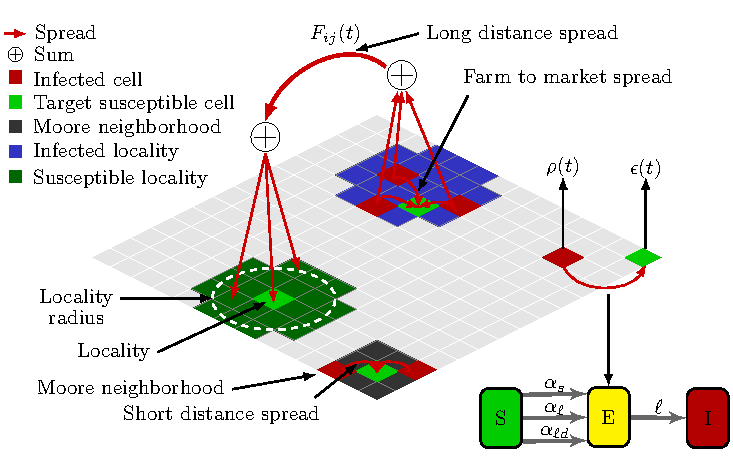
\includegraphics[width=\textwidth]{figs/model_schematic.pdf}
    \caption{\label{fig:modelConcept}}
    \end{subfigure}
    \begin{subfigure}[b]{.37\textwidth}
    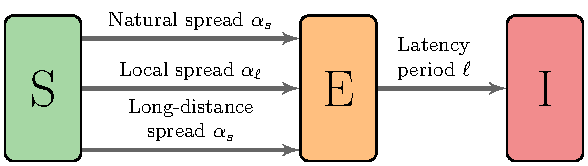
\includegraphics[width=\textwidth]{figs/SEI.pdf}
    \caption{\label{fig:SEI}}
    \end{subfigure}
    \caption{\textbf{Schematic of the model.} (a)~The multiple pathways of
    spread are illustrated. (b)~The states and factors that influence state
    transitions.}
\end{figure}
%%

\subsection{\tuta{} biology}
\label{sec:biology}
The tomato leafminer exhibits a short life cycle of about 24--38 days
(temperature at $25\pm3^\circ$C), from egg to adult, as it is a
multivoltine species with overlapping generations in the
field~\cite{guedes2012tomato}. This species causes serious damage to
numerous solanaceae crops such as eggplants, potatoes, and especially
tomato crops~\cite{sylla2018}. It penetrates into tomato leaves, stems, or
fruits, wherein it feeds and develops by creating conspicuous mines as well
as galleries. \tuta{} additionally restricts tomato plant growth by feeding on
the growing tips. Considering the warm weather throughout the year,
particularly in the dry season, the study region presents ideal conditions
for rapid development and spread of \tuta{}. Pest risk
analysis~\cite{tonnang2015identification} shows that the Ecoclimatic Index
for this region is above~$50$ (highly suitable). Sylla et
al.~\cite{sylla2018} analyzed host preference of~\tuta{} in France and
Senegal. While the highest preference is for tomato, it can survive well on
eggplant and potato, which happen to be major vegetable crops in the study
region. However, since \tuta{} primarily attacks leaves of eggplant and
potato, the chance of the pest spreading through trade of these crops seems
to be low. 
%%
\subsection{Model description}
\newcommand{\pshort}{p_s}
\newcommand{\plocal}{p_{\ell}}
\newcommand{\pld}{p_{\ell d}}
\newcommand{\asd}{\alpha_s}
\newcommand{\afm}{\alpha_{\ell}}
\newcommand{\ald}{\alpha_{\ell d}}
\newcommand{\produce}{\mathrm{Prod}}
\newcommand{\veg}{\mathrm{V}}
\newcommand{\temp}{\mathrm{T}}
\newcommand{\consume}{\mathrm{Cons}}
\newcommand{\locality}{\mathrm{L}}
\newcommand{\export}{\mathrm{Export}}
\newcommand{\import}{\mathrm{Import}}
\newcommand{\process}{\mathrm{Proc}}
\newcommand{\moore}{\mathrm{M}}
\newcommand{\mooreRange}{r_\mathrm{M}}
%%
We use a discrete-time Susceptible-Exposed-Infected (SEI) epidemic model to
simulate multi-pathway pest dispersal. See Figure~\ref{fig:modelConcept}
for an illustration. The focus region is overlayed with a grid of cell
size~$0.25$ arc degree $\times 0.25$ arc degree, which is
approximately~$27.8\mathrm{km}\times\mathrm{27.8km}$ at the equator. These
dimensions are comparable to that used in Guimapi~et.~al.~\cite{guimapi2016modeling}
($25\mathrm{km}\times25\mathrm{km}$). Each cell can be in three states:
susceptible ($S$) denoting pest free state, exposed ($E$) denoting that the
pest has been introduced but the population has not yet built up to
influence other cells, and infectious ($I$) denoting that the pest has
established and the cell can influence its neighbors (in each pathway).
The simulation progresses in
discrete time steps, where each step corresponds to a month. The likelihood
that a cell transitions from state~$S$ to~$E$ depends on (i)~suitability of
the cell for \tuta{} to establish at that time step, (ii)~influence of cells
in state~$I$ in each pathway, and (iii)~level of infestation in each cell
with state~$I$. An exposed cell goes to the state~$I$ after a latency
period of~$\ell$ time steps. This is the time required for the population
to build up to infect other cells.

\paragraph{State transitions.} The rules for state transitions are shown in
Figure~\ref{fig:SEI}. A susceptible ($S$) cell can be influenced by
infectious (state~$I$) cells through the three different pathways. Each
such cell infects the susceptible cell with some probability. If \tuta{} is
succesfully introduced to a cell, it moves from state~$S$ to~$E$. The
exposed state corresponds to the situation where \tuta{} has established,
but it is not widespread in the area to influence other cells. It stays in
state~$E$ for one time step before transitioning to state~$I$. This is a
reasonable assumption considering that the conditions are favorable for the
pest to complete a life cycle within one month. Once the pest has
established in a cell, the cell remains infected forever, a fair assumption
considering that, historically, eradication of \tuta{} has not been
successful\footnote{The only exception is United Kingdom where the pest was
detected early~\cite{cabiUK}.}.
%%
%% \begin{figure}[ht]
%%     \centering
%%     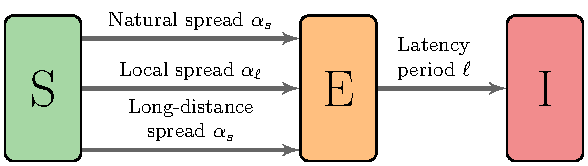
\includegraphics[height=.16\textwidth]{figs/SEI.pdf}
%%     \caption{Schematic of the SEI process.\label{fig:SEI}}
%% \end{figure}
%%

\paragraph{Susceptibility and infectiousness of a cell.} We have used
monthly production to determine the susceptiblity of a cell in state~$S$
and infectiousness of a cell in state~$I$. The suitability of a cell~$v$
for pest establishment at time~$t$ is denoted by~$\suitable(v,t)$. This
is~$1$ if production at~$t$ is non-zero and~$0$ otherwise.  For a cell in
state~$I$, the level of infestation in an infected cell~$v$ at time~$t$ is
denoted by~$\infest(v,t)$. It is modeled as a linear function of host
presence at time~$t$, for which we use the weighted sum of production
volume of tomato, eggplant, and potato in that cell
at time~$t$. The weights correspond to relative oviposition preference of
\tuta{} on the three hosts.

\paragraph{Localities.} To account for human-assisted dispersal, we
considered dense centers of human activity such as big cities or towns.
Typically, these locations are the major consumers of vegetables. Since
horticultural products are less durable, in developing countries, owing to
lack of good storage and transport infrastructure~\cite{ali2001}, major
producing regions are close to cities~\cite{buckmaster2014going}. In
addition, they house big wholesale markets and the trader and distributor
infrastructure. Therefore, capturing the spread due to activities within
and between cities is critical to model human-mediated spread. For this
purpose we constructed \emph{localities}, each representing dense pockets
of human activity in the following manner.  We identified major urban
centers in the study region. A \emph{locality} corresponding to each city
consists of all grid cells for which this is the nearest city and the
distance is at most the \emph{locality radius} (in kilometers), with the
additional constraint that each cell belongs to the same country as this
city. We also account for administrative restrictions. Local human-mediated
dispersal is modeled as the interaction between cells belonging to a city.
Long distance human-mediated dispersal is modeled as trade flows of
considered host crops from one city to another. For a
city~$i$,~$\locality(i)$ denotes all cells which are assigned to it.
%% Each cell~$v$ has the following time varying attributes: \aacomment{these
%% are not necessary: NDVI~$\veg(v,t)$,
%% temperature~$\temp(v,t)$,} monthly production of preferred host crops and
%% consumption~$\consume(v,t)$, where~$t$ corresponds to a month.
%% \aacomment{This should get into Tonnang discussion: Since NDVI
%% data is available at a much finer resolution (see Table~\ref{tab:data}),
%% for each cell, we assign the maximum of the NDVI data points that fall in
%% this cell for that month.} For production, we consider the following
%% vegetables: tomato, potato, eggplant in metric tonnes (see
%% Section~\ref{sec:biology} on choice of host crops). Annual country-level
%% production data (in volume) is spatially disaggregated using SPAM data
%% on spatial distribution of vegetable production. \aacomment{needs
%% explanation. statistical analysis should come here}. Further, for each cell,
%% this production was distributed temporally-- one value for each month of
%% the year. We observed that precipitation is a primary driver of production
%% in the study area; during wet months, the amount of production is
%% considerably less. \aacomment{statistical analysis should come here} (See Supplementary Information).
%% \aacomment{pending: consumption, import/export}

Now, we describe the three different pathways of spread.
\paragraph{Short distance dispersal.}
At any time step, a cell's state is influenced by its Moore
neighborhood of range~$r$. When range~$r=1$, it corresponds to the
adjacent cells (eight at most) and when~$r=2$, it corresponds to~$r=1$
neighbors and cells adjacent to them. The Moore neighborhood of~$v$ is
denoted by~$\moore_v$.
\begin{align}\label{eqn:pshort}
    \pshort(v,t)=\asd\suitable(v,t)\bigg(1-
    \exp\Big(-\sum_{v'\in\moore_v(r)}\infest(v',t)\Big)\bigg),
\end{align}
where~$\asd$ is a tuning parameter for this pathway. The probability
that~$v$ is influenced by its neighbors is
$1-\prod_{v'\in\moore_v(r)}1-\infest(v',t)$, which is approximated
by equation~\eqref{eqn:pshort}.
%%
\paragraph{Local human-mediated dispersal.}
Here, the cell's state is influenced by the infected cells in its locality
through the marketing chain.  In general, it is hard to model the local
dynamics as there are several actors in bringing the commodities from farm
to market to consumers.  Further, these are country and commodity specific.
See for example Kethonga~et~al.~\cite{kethonga2004} for the typical
structure of marketing chains and Rebaudo~et~al.~\cite{rebaudo2011} for
modeling human interactions in the context of invasive species spread.
Here, we use a simple approach. Every cell~$v$ is influenced by cells in
its locality~$\locality$ based on their infectiousness. 
The expression is similar to that in~\eqref{eqn:pshort}, but with cells in
the locality instead of the Moore neighborhood.

%%
\begin{align}\label{eqn:plocal}
    \plocal(v,t)=\afm\suitable(v,t)\bigg(1-
    \exp\Big(-\sum_{v'\in\locality}\infest(v',t)\Big)\bigg),
\end{align}
where~$\afm$ is a tuning parameter for this pathway.
%%
\paragraph{Long-distance human-mediated dispersal.}
%%
We only consider trade of tomato in our model (see
Section~\ref{sec:biology}).  We model the flow of vegetables among markets
based on the following assumptions: (i)~the total outflow from a city
depends on the amount of produce in its surrounding regions and imports
from countries outside the focus region at time~$t$, and (ii)~the total
inflow depends on total consumption, processing demand, and exports from
the city to countries outside the focus region. For each country, the
domestic flow is estimated using a doubly constrained gravity
model~\cite{kaluza2010complex,anderson2011gravity}. For a city~$i$,
let~$O_i$ and~$I_i$ denote total outflow and total inflow respectively.
The flow~$F_{ij}$ from city~$i$ to city~$j$ is given by
%%
\(
   F_{ij}(t)=a_i(t)b_j(t)O_i(t)I_j(t)f(d_{ij}),
\)
%%
where, $d_{ij}$ is the time to travel from~$i$ to~$j$, and $f(\cdot)$ is
the \emph{distance deterrence function}:
$d_{ij}^{-\beta}\exp(-d_{ij}/\kappa)$, where~$\beta$ and~$\kappa$ are
tunable parameters. The
coefficients~$a_i$ and~$b_j$ are computed through an iterative process such
that the total outflow and total inflow at each node agree with the input
values~\cite{kaluza2010complex}. Overall, we have~12 networks
representing flows for each month. The outflows and inflows are calculated
as follows:
%%
\begin{align}\label{eqn:flow}
    O_i(t)&=\produce(i,t)+\import(i,t)-\export(i,t)-\process(i,t),\\
    I_i(t)&=\consume(i)\,.
\end{align}
Here,~$\produce(i,t)$ and~$\consume(i)$ are the monthly production and
consumption (assumed same every month) at the locality.  $\export$ and
~$\import$ are the monthly total export to, import from or both from outside the
country.  $\process(i,t)$ is the
tomato produced for processing. Typically, tomato meant for
processing is cultivated locally~\cite{wijk2007}. In the
next section, we will discuss how each of these locality attributes are
computed.  Given a locality~$j$, let its total infectiousness be denoted
by~$\totinf(j,t)=\sum_{v'\in\locality(j)}\infest(j,t)$. Suppose cell~$v$
belongs to locality~$i$. Then, the probability of cell~$v$ transitioning
from~$S$ to~$I$ due to long-distance dispersal is given by:
%%
\begin{align}\label{eqn:plocal}
    \pld(v,t)=\ald\suitable(v,t)\bigg(1-
    \exp\Big(-\sum_{j\ne i}\sum_{v'\in\locality(j)}F_{ji}\totinf(j,t)\Big)\bigg).
\end{align}
%%
Here,~$\ald$ is a tunable parameter for this pathway and~$i$ is the
locality to which~$v$ belongs to. The influence depends
on total infectiousness of a locality and the flow from that locality to
the locality~$i$.
%%
\subsection{Cell, locality, and network attributes}
%%
In this section, we will describe how attributes such as production,
consumption, and trade flows between localities were computed.
Table~\ref{tab:data} provides the list of model parameters with their
values or ranges and data source as applicable.

\paragraph{Seasonal production.}
Broadly, in this region, the cropping pattern depends on two factors:
seasons--dry and wet, and elevation--highland (upland) and lowland. 
The aim was to estimate monthly production volume of tomato, eggplant and
potato for each cell. This was accomplished in two steps. First,
we estimated annual production in each cell. Then, this value was
disaggregated to monthly production. The annual production was estimated as
follows. From SPAM~\cite{spam}, we obtained annual production
estimates for each cell. However,
there are several issues with directly using this data. Firstly, these are estimates
for the year~$2005$, and secondly, tomato and eggplant production estimates
are not available. Instead, vegetable production volume is
available. Also, for countries where data was available, we did not find any correlation between reported tomato
(eggplant) production and total SPAM vegetable production for that region. Therefore, for each country, we obtained the most recent
production data available (2013 or later) at the highest spatial
resolution (region/province/country) (Table~S1). The production of a particular
vegetable type at a cell was computed
as follows: 
%%
\[\frac{\text{Total production in the region}}{\text{Total SPAM production
    for cells in the region}}\times \text{SPAM production in the cell}\].
%%
For tomato and eggplant, we used vegetable production as the surrogate.
There were also cases where no data was available (Cambodia, Myanmar and
Laos for example). In such cases, for potato, we used SPAM data as is. For
tomato and eggplant, the SPAM value for vegetables was scaled by a scaling
factor which was determined as follows. For countries where data was
available, we computed the ratio of total tomato production and total SPAM
vegetable production for the country. The median value ($\approx0.05$) was
used as the scaling factor. The same procedure was used for eggplant. 

To predict seasonal production, we used regional quarterly tomato and
eggplant production data that was available for Philippines~\cite{psa} (16
regions), precipitation and elevation data at the cell level. For each
region, we obtained the product rate by normalizing quarterly production
values with respect to maximum value among these. We used production rate
instead of production values since there are several factors that determine
a region's production: climate, vegetable preference, demand, etc.
Therefore, it may not be meaningful to compare production across regions.
We conducted a linear regression with the product rate as a dependent
variable and precipitation and elevation as independent variables
(SPSS~24.0). Since the dependent variable was highly skewed, we used a
log-transformation. To control elevation, we classified the elevations into
two groups, high and low, using $k$-means clustering (SPSS~24.0). Due to
the small sample size, we excluded the samples in the high-elevation group
and conducted a linear regression analysis for the group of low
elevation~($< 235$). The total 56 samples in the group showed negatively
strong correlation between precipitation and logarithm of product rate
($r=-0.734$). More information is provided in Supplementary Information.
For most countries, only qualitative information on seasonal production is
available making validation near impossible.  However, we observed that for
the entire region seasonal production was strongly tied to rainfall; during
the wet season, the amount of production is considerably less compared to
the dry season.

%% on data availability. The first method was used if only seasonal
%% production is available for a region or country. In this case, we first
%% estimated seasonal production in each cell and then disaggregated it
%% to obtain monthly production. Here, due to unavailability of data for tomato and eggplant, we used SPAM's total
%% vegetable production as surrogate. To disaggregate into monthly production,
%% we studied the relationship between production, precipitation, and elevation.
%% For lowland areas, %(elevation less than ???) 
%% production is negatively
%% correlated with precipitation ($r<-0.75$).

\paragraph{Locality construction.}
We identified cities with population greater than a certain population
threshold in the entire study region to determine localities in the model.
We considered a range of threshold values, and chose~$250,000$ as the
threshold for the model with the main criteria for the choice being
coverage of production and population, and knowledge of major wholesale
markets (Supplementary Information). The locality radius was chosen to
be~$100$kms since local production in an urban area was within 50--60kms
from the city center (Table~S2, Supplementary Information). To obtain long
distance trade flows, the travel times between pairs of cities were
computed using Google API~\cite{googleapi}. For the distance deterrence
function of the gravity model, we set~$\beta=2$ and~$\kappa=300$ (kms). The
former was set based on the analysis in
Venkatramanan~et~al.~\cite{venkatramanan2017towards} while for the latter
we observed from literature survey that long distance trade is typically between
nearby towns.

\paragraph{Production, consumption, imports, exports and processing.}
Monthly tomato production at a locality was obtained by aggregating
production at all cells that belong to it. For consumption, we used
country-level production~\cite{consumption}, which was available for half
of the countries. For Singapore, we estimated it as the difference between
total inflow (production and imports) and total outflow (exports) based on
FAO data. For Vietnam, Wijk~et~al.~\cite{wijk2007} provides this
information. For Myanmar, Cambodia and Laos, we found no information. We
used median consumption for the region. We also analyzed consumption with
respect to per capita gross domestic product (GDP). However, we did not
find any correlation between GDP and consumption both globally as well as
restricted to the study region. 

For most countries, imports and exports are a small fraction of domestic
production. We have ignored these quantities.  However, these flows were
accounted for when evaluating possibility of pest introduction. The main
exceptions were the significant tomato imports from India to Bangladesh and
trade between Malaysia and Singapore. We identified major routes of trade
from India to Bangladesh~\cite{EIIndia2015} and the total imports from
India (FAOSTAT) was distributed uniformly between three cities close to the
border with India along these routes. Finally, these imports were evenly
distributed for the later half of the year since Bangladesh imports mostly
during the rainy season. To capture the significant trade between Singapore
and Malaysia, we included Singapore in the domestic flow network of
Malaysia as there is high interaction between the two countries.  The
resulting flow from the gravity model from Malaysia to Singapore was
obtained by aggregating network flows across months and across edges with
Singapore as destination.  This flow was comparable to the annual imports
from Malaysia to Singapore. With the exception for
Thailand~\cite{mict2013}, there is no information on the amount of tomato
production consumed by the processing industry even though there is
evidence of processing industry in Vietnam~\cite{wijk2007}, Malaysia and
Indonesia. For each locality in Thailand, we scaled the monthly production
by the ratio annual production of fresh tomatoes over total annual
production (fresh and processed).

%% \paragraph{Network structure.} The resulting network consists of~$8,010$
%% cells and~$109$ localities.  
%%
%%
\begin{table}[t]
    \caption{Model parameters and variables, their ranges and references.\label{tab:data}}
    \centering
	\small
    \begin{tabular}{l p{4cm} p{3cm} p{5cm}}
    %{cp{.25\textwidth}p{.25\textwidth}lr}
		\hline		
		Parameter & Description & Range/values & Source \\
\hline		
\hline
$\mooreRange$ & Range of Moore neighborhood & 1,2,3 &
\cite{guimapi2016modeling}\\
$\ell$ & Latency period to transition from $E$ to $I$& 1,2,3 & \\
\hline
$\beta, \kappa$ & Gravity model parameters & 300--500,2 &
\cite{venkatramanan2017towards}\\
-- & Locality population threshold and radius & 250,000, 100kms &
population of cities~\cite{citypop} and reports\\
\hline
$\suitable$ & Suitability threshold & 0\\
$\infest$ & Infectivity of a cell based on amount of production & & Host
production (SPAM), host preference~\cite{sylla2018}, precipitation and
elevation \\
\hline
Scenarios & Seeding simulations: time and cells to infect & 4 cases:
Bangladesh (B1 and B2), Malaysia (M1) and Philippines (P1) & \tuta{} incidence
reports in Bangladesh, FAOSTAT for international trade and migration
reports.\\
Start month & & March, April, May & Based on incidence reports\\
\hline
$\asd$ & Short-distance spread scaling factor & 0--500\\
$\afm$ & Local human-mediated dispersal scaling factor & 0--500\\
$\ald$ & Long distance spread scaling factor & 0--500 \\
\hline
%% 		& Tomato production & & & FAOSTAT  \\	
%% 		& Vegetable production distribution & & & SPAM  &5 min. $\times$ 5 min. & \\	
%% 		& Production seasonality & & & &Country level, Monthly &    \\
%%         \hline
%% 	    & Tomato consumption & & & FAO & 
%%         Country, Annual & 2011 \\	 
%% 		& Population & & & Landscan & 0.008333 $\times$ 0.008333 degrees &   \\
%%         & Per Capita Income & & & FAO\aacomment{check}
%% 		& Country & 2013 \\
%%         \hline
%% 	    & Tomato import/exports & & & FAOSTAT &Country, Annual& 2013 \\
%% 		& Cities and their population & & & MAXMIND &City/town & 2017  \\
%% 	    & City distances & & & Google Maps, Distance matrix API & City & 2017  \\
%%         \hline
%% 	    & \tuta{} incidence reports & \\
%% 		\hline
    \end{tabular}
    %% \newline
    %% $^\dagger$The appropriate references are provided in the Supplementary
    %% Information.
\end{table}


\subsection{Experiment design}
\label{sec:expDesign}
The tunable parameters of the model are the pathway scaling
factors~$\asd$,~$\afm$, and~$\ald$, Moore range~$\mooreRange$, latency
period~$\ell$ and the scenario , i.e., start point of infestation (time and
location). These are listed in Table~\ref{tab:data}. First, we simulated
the spread in Bangladesh where \tuta{} is already present and incidence
reports are available. We evaluated the model output for each set of
parameter values by comparing it with ground truth using a maximum
likelihood estimation method for comparison. We used a sparse adaptive
design with refinements using Classification and Regression Trees (CART)
method to parameterize the model. The selected model was subsequently used to study
the possible spread in the rest of the region under various scenarios.
Sensitivity analysis was performed to assess uncertainty of model outcomes.

Evaluation of the model is a particularly challenging task as available
incidence data is highly inadequate for calibration and validation. For
example, there are only eight locations in Bangladesh for which data is
available. Further, it is possible that there were delays in identifying
and reporting.  Therefore, during the model evaluation phase, to account
for both spatial and temporal observation noise, we considered six
scenarios: Start times were March, April or May (the month \tuta{} was
reported) and two locations of initial infections (i)~B1: cell
corresponding to location of first report ($26.19^\circ$N, $88.43^\circ$E)
and (ii)~B2: all cells in the Moore neighborhood (range~1) for the location
of first report.  For each parameter setting the simulation was run with
100 repetitions.  We computed the empirical probability that a cell is in
state~$I$ at time~$t$.  The output was compared with ground truth using a
maximum likelihood method adapted
from~\cite{carrasco2010unveiling,keeling}. Let~$C$ be a reporting cell
with~$t_C$ denote the month of actual report. To account for uncertainty in
reporting, we consider a time window rather than the exact time of report
during comparison. Let~$U_\tau=[t_C-\tau,t_C]$ be the time window or
interval, where~$\tau$ is the uncertainty parameter. Here, for simplicity,
we will assume that~$t_C$ is greater than or equal to~$\tau$.
Supposing~$\reportingCells$ is the set of cells corresponding to ground
truth,  and ~$p(C,t)$ is the probability that cell~$C$ is infected at
time~$t$ in the model, then, the likelihood~$\likelihood$ is given by,
\[
    \likelihood=\sum_{C\in\reportingCells} \Big(\sum_{t\in U_\tau}p(C,t)
    + \sum_{t\notin U_\tau}\big(1-p(C,t)\big) \Big)
\]
In our case, the uncertainty parameter~$\tau=2$.  First, we coarsely
sampled the parameter space. Applying CART, we identified subspaces of the
parameter space for which likelihood was high (see Figure~\ref{fig:cart}).
We refined our search in the next stage to improve the parameterization.
In addition, we implemented the cellular automata model by
Guimapi~et~al.~\cite{guimapi2016modeling} which serves as the baseline
model for comparison.

\paragraph{Software and Computational aspects.} The model was implemented
in Python~2.7. For data management and processing, we used PostGreSQL and
SQlite.  Statistical analysis was done using Python, R~3.4.3 and SPSS~24.0.
The experiments were run using Discovery, a high performance computing
cluster with 232 nodes (16-core Sandy Bridge-EP E5-2670 2.60GHz (3.30GHz
Turbo) Dual Processor (8 Cores per Processor) nodes with 32 GB of Memory
and 500 GB Internal Hard Drive).

%%
\section{Results}
%%
\subsection{Production, trade and pathways of pest entry in the study region} 
\label{sec:entry}
Using data from FAO (FAOSTAT 2013, Table~\ref{tab:data}), we analyzed the
dynamics of production and trade of various hosts of \tuta{}.
Here, the objective is to study the dynamics of country-level production
and trade flow of various hosts of \tuta{}.
%%
\paragraph{General trends.} 
A plot of normalized aggregated tomato production, imports, and exports in
the region is shown in Figure~\ref{fig:trends} (Supplementary Information). There is a steady increase in the production
and amount of internal trade, with more or less the same rate of change for
both quantities.  While the export of tomato outside of the focus region
(plot ``Exports'') has risen steeply in the recent years, the imports
generally indicate a downward trend (plot ``Imports''). However, there is a
lot of discrepancy in reporting import (or export) figures, particularly
the commodity flows with countries outside the region. The filled curves
shows the difference in these estimates when considered individually.
However, the plots clearly indicate that there is a general thrust towards
tomato production and trade in the region. Recent efforts to
increase production and trade infrastructure in these countries endorse
this increasing trend~\cite{}. Under these circumstances, \tuta{}'s
invasion can have a high negative impact on the economy and livelihood of
the people in this region.
%%
\begin{figure}[ht]
\centering
%%
\begin{subfigure}[b]{.45\textwidth}
    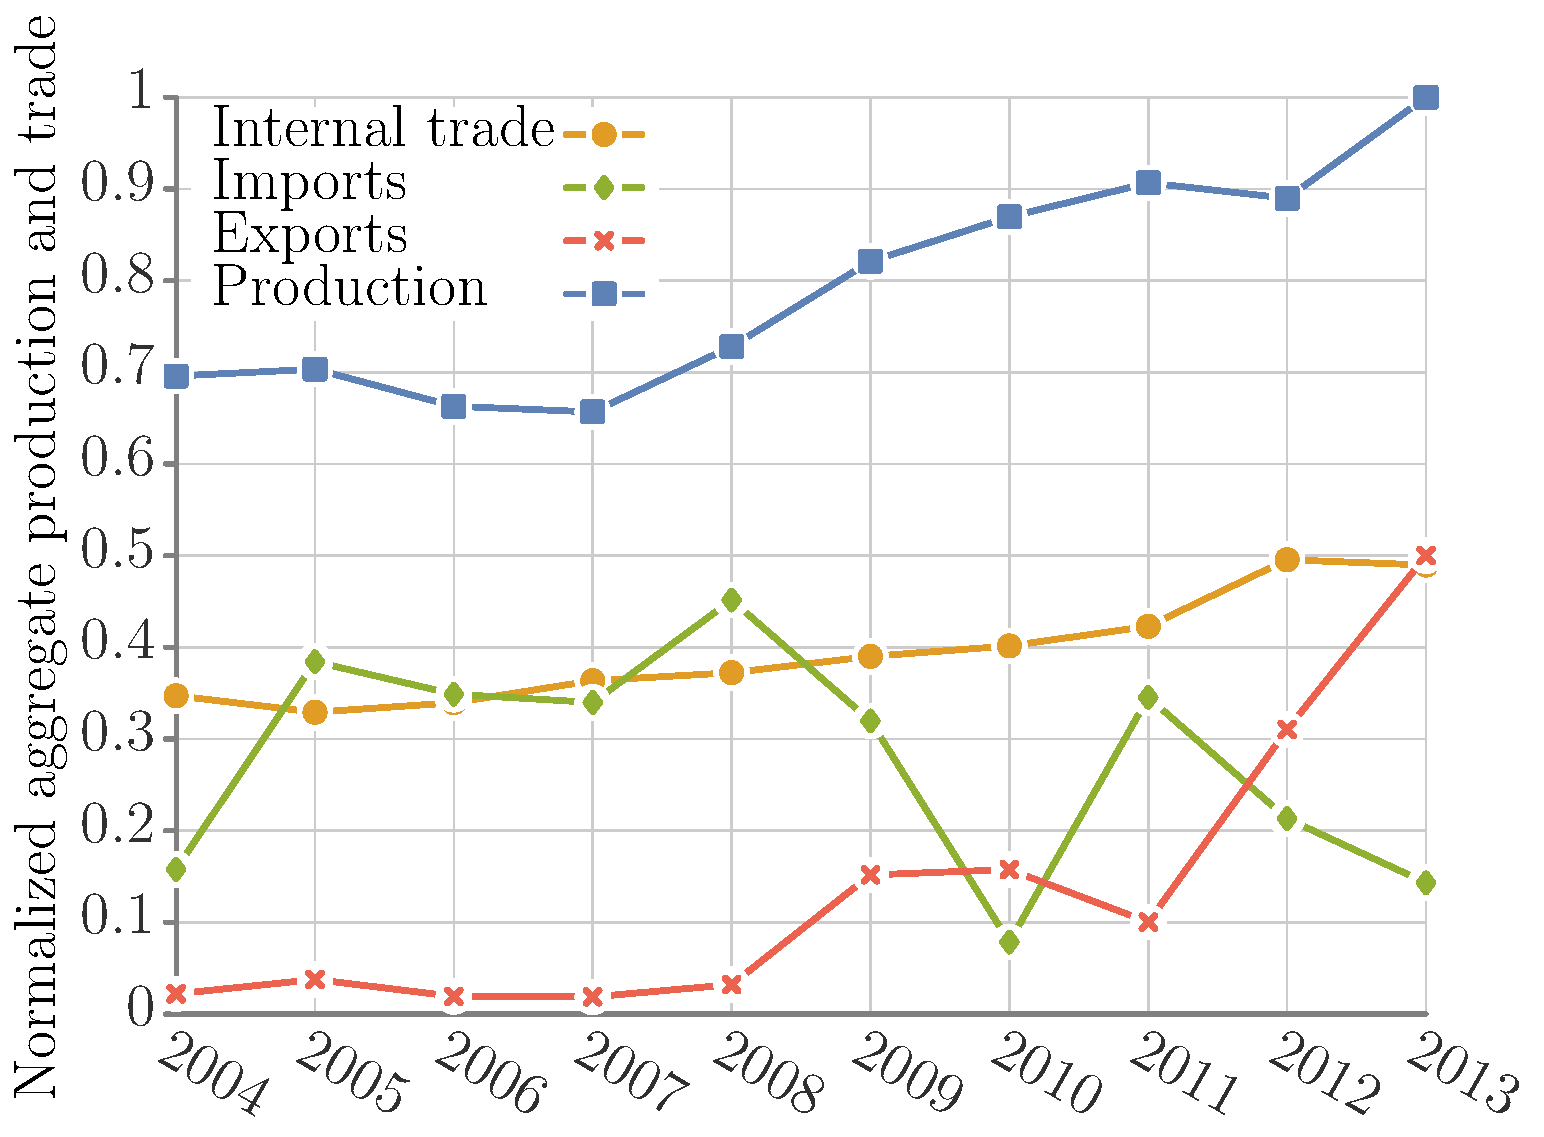
\includegraphics[width=\textwidth]
    {../international_trade/results/stat_plots/trends.pdf}
    %{figs/trends.pdf}
    \caption{\label{fig:trends}}
\end{subfigure}\hspace{.5cm} 
%%
\begin{subfigure}[b]{.45\textwidth}
    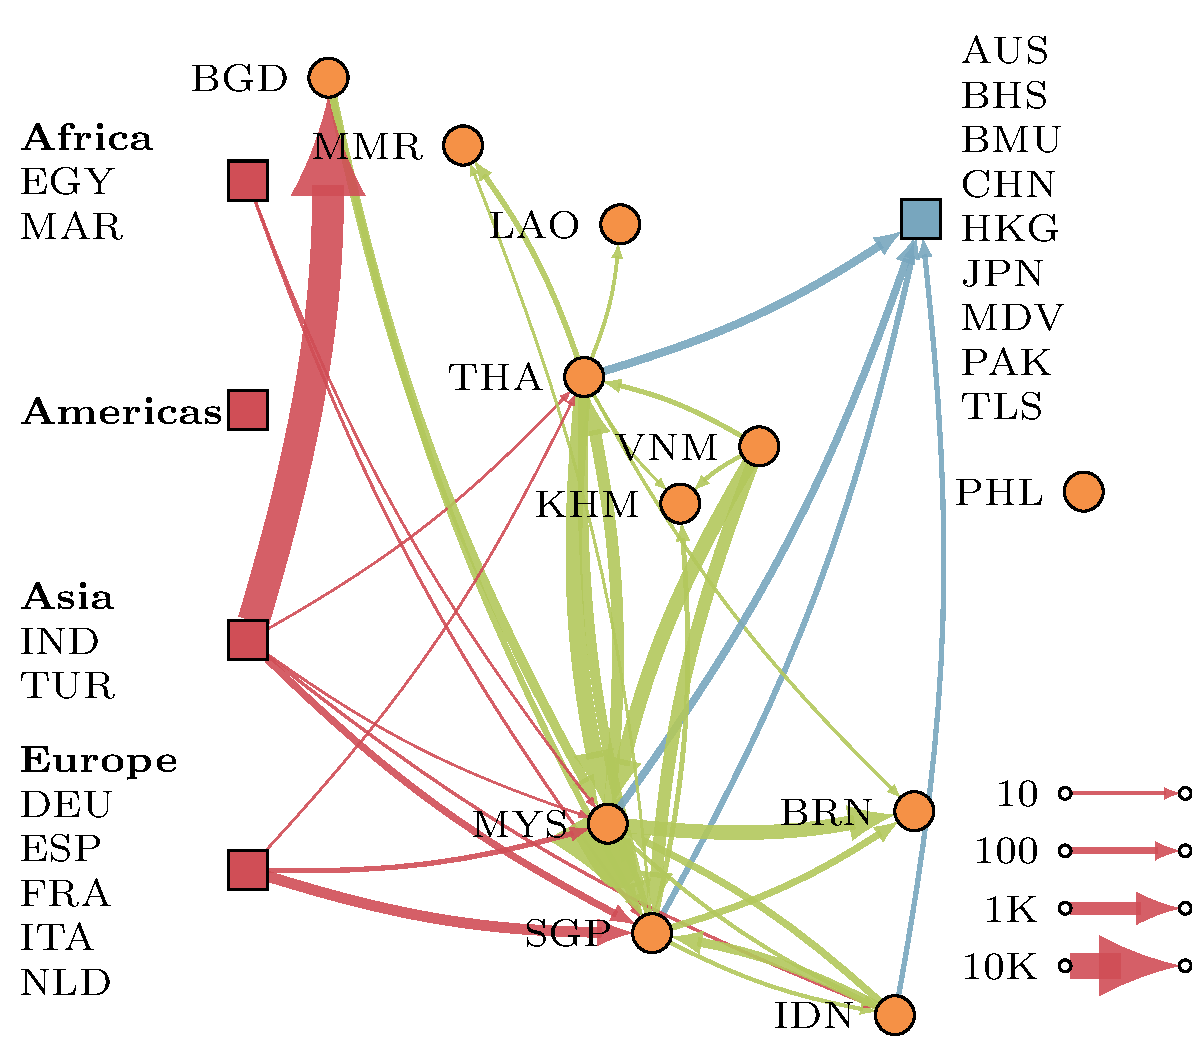
\includegraphics[width=\textwidth]{../international_trade/results/network_plots/sea_2013_tomato.pdf}
    \caption{\label{fig:tomnet}}
\end{subfigure}
\caption{\textbf{Country-level production and trade of tomato in the focus
region using FAOSTAT 2013.} (a)~General trends of overall production and
trade in the region over a decade. We aggregated tomato production across
countries in the region for each year from~2004 to~2013 and normalized by
dividing it by the maximum value. We did the same with imports into and
exports out of the region as well as internal trade. The trade data
presented for each year is the average of total quantity reported by
importing countries and exporting countries. (b)~The trade of tomato in the
focus region. The trade between countries of the focus region is
represented by green edges.  Also shown are imports from \tuta{} affected
countries categorized by region. The edge thickness is a function of the
trade volume.}
\end{figure}

\paragraph{Production.}
Among the countries listed in the FAOSTAT dataset, Indonesia is by far the
largest producer ($\approx1$M tonnes) followed by Phillipines and Malaysia
($\approx200$K tonnes each).  FAOSTAT does not have tomato production data
for Vietnam and Cambodia.  However, alternate data sources (personal
communication) indicate that Vietnam is the second largest producer
($\approx400$K tonnes) (see~\cite{vien2006overview} for 2005 information).
The data also indicates that Indonesia is the largest producer of eggplants
in the region, followed by Philippines.

\paragraph{Trade.}
The network capturing tomato trade within the focus region, imports from
\tuta{} affected countries and exports to countries which have not reported the
pest, is shown in Figure~\ref{fig:tomnet}. The network was constructed
using data from FAOSTAT Trade matrix (Table~\ref{tab:data}). We note that
with the exception of Philippines, there is a lot of trade activity among
countries in the focus region. However, the majority of trading happens
between neighboring countries. Malaysia and Singapore serve as major hubs
for tomato trade with considerable amount of trade among themselves, within
the focus region and beyond. Most significant flows are from Malaysia to
Singapore ($>30,000$ tonnes) followed by Thailand to Malaysia ($>2,000$
tonnes).  Philippines does not report any fresh tomato trade with other
countries.  However, it does report imports of processed tomato~\cite{}. We
also analyzed how the network structure evolved across years. While we did
not observe much variation in the network structure, there is some change
in the countries importing to and exporting from this region (Supplementary Information for networks of alternate hosts).
%%
\paragraph{Pathways of entry.} \tuta{} was first reported in northern
Bangladesh near Rangpur (Table~S3).  Since then it has spread to almost all
major tomato producing areas of the country. The pest could enter the study
region from Bangladesh to neighboring countries such as Myanmar. In fact,
our analysis (Section~\ref{sec:predict}) indicates that there is a high
chance that the pest is already present in this country. Also, the network
structure does indicate a high risk of introduction of \tuta{} through
trade. In particular, our analysis of how the network has evolved over the
years (Supplementary Information) shows that while the basic network
structure does not vary much, the imports from \tuta{} infested countries
is steadily increasing.  By virtue of being important hubs, there is a high
chance that the pest will enter through the ports of Malaysia and
Singapore, and spread to Thailand, Brunei, and Indonesia due to their high
interactions with these neighbors. Since Philippines does not share its
borders with any country in the region and there is no evidence of tomato
trade with rest of the countries, there is a low chance that the pest will
be introduced through natural spread or trade.  However, human mobility is
a possible pathway. The Middle East is the top destination for Filipino
workers~\cite{rodriguez2011philippine}. Therefore, there is a possibility
of introduction through travel. Besides, it is possible that this was the
case with India. In~2014, \tuta{} was reported in the South Western part
much farther away from the country's border with its neighbor Pakisthan
which is yet to report presence of the pest.  Afghanisthan reported only
in~2015. Also, India does not show any imports from \tuta{} infested
countries.
%%
\subsection{Assessing the role of each pathway in the spread of \tuta{}}
In Bangladesh, following the first report of \tuta{} in India in
2014~\cite{kalleshwaraswamy2015occurrence}, pheromone traps were deployed
in eight places (Table~S3). In May~2016, the
pest was detected in Panchagarh District in the northern part of
Bangladesh~\cite{hossain2016first}. Within~10 months, the pest was reported
in almost all major areas of vegetable production.
Our analysis strongly indicates that both short distance spread and trade
are important pathways in the spread dynamics. For the parameter set with
the best fit, the likelihood was close to~$6$, i.e., on an average,
simulation output matched six out of seven locations. If we consider the
case where the human-influence was turned off ($\afm=0$ and~$\ald=0$), the
highest likelihood was~$5$. Also, we observed an interesting pattern with
respect to Moore range ($\mooreRange$) and latency period ($\ell$). When
only natural spread is considered, the rate of expansion is higher
($\mooreRange=2$) and latency period ($1$) is lower than when we account
for human-mediated spread ($\mooreRange=1,\ell=2$).  This is in some sense
expected due to long distance jumps facilitated by human-assisted spread.
It also means that \tuta{} can achieve the same (or greater) range
expansion with considerably less flying capacity and population growth.

While our results highlight the role of human-mediated spread, it is
possible that this pathway is more important for the spread than it
appears.  First of all, vegetable production data for Bangladesh (SPAM)
indicates that almost all cells have non-zero production of hosts of
\tuta{}. Therefore, there is a contiguous landscape of suitable areas for
the pest to spread naturally. But in general this may not be the case; the
only way two locations can be connected is by trade or travel pathways. One
obvious example is two land masses separated by sea.  Secondly, and more
importantly, it does not explain the gap between the first report and the
report in Gaibandha district ($25.15^\circ$N, $89.23^\circ$E, Table~S3
in Supplementary Information). The distance between the two locations is
only $185$kms while this location reported the presence only after nine
months of first report suggesting that natural spread might be much slower.
According to our best fit model accounting only for natural spread, the
corresponding cell gets infected between the third and fifth months.

We simulated the spread using the model developed by
Guimapi~\cite{guimapi2016modeling} for Bangladesh.  For Moore neighborhoods
of~2 and~3 the spread was too rapid (likelihood~$1$), indicating that the
spread might be slower than what is predicted by the model.

%%
\begin{figure}[ht]
    \centering
    \begin{subfigure}[b]{.48\textwidth}
    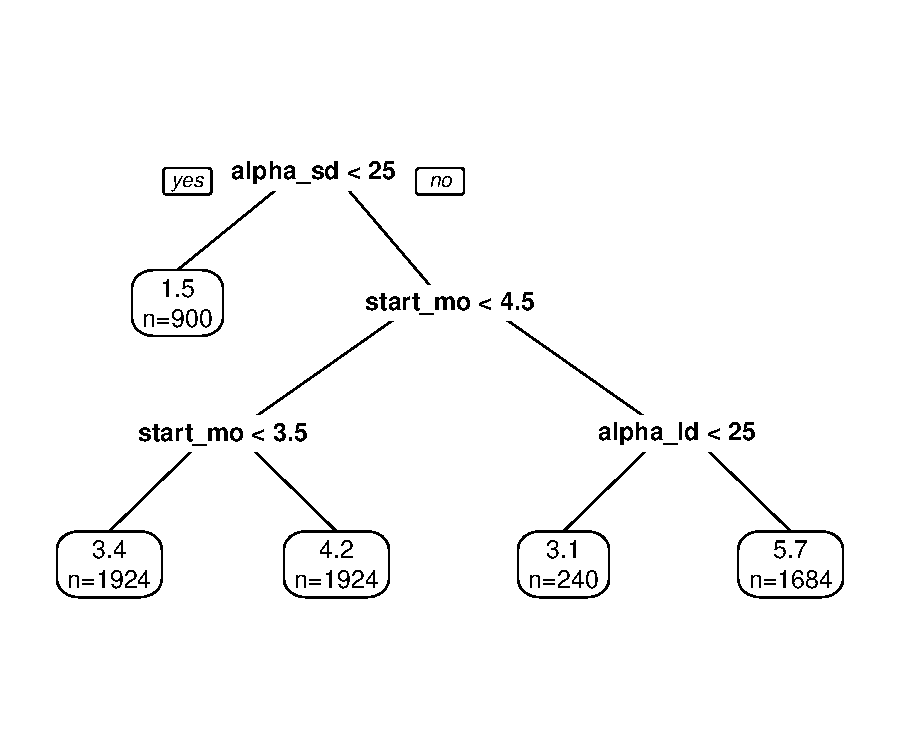
\includegraphics[width=\textwidth]{figs/cart_analysis1.pdf}
    \caption{\label{fig:cart1}}
    \end{subfigure}
    \begin{subfigure}[b]{.48\textwidth}
    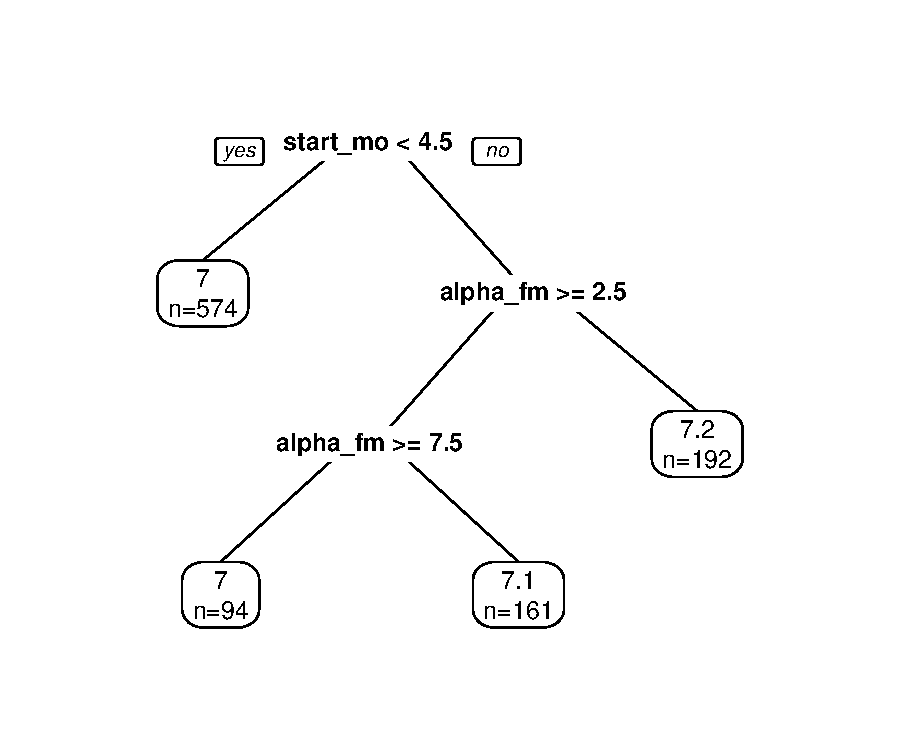
\includegraphics[width=\textwidth]{figs/cart_analysis2.pdf}
    \caption{\label{fig:cart2}}
    \end{subfigure}
    \begin{subfigure}[b]{.48\textwidth}
    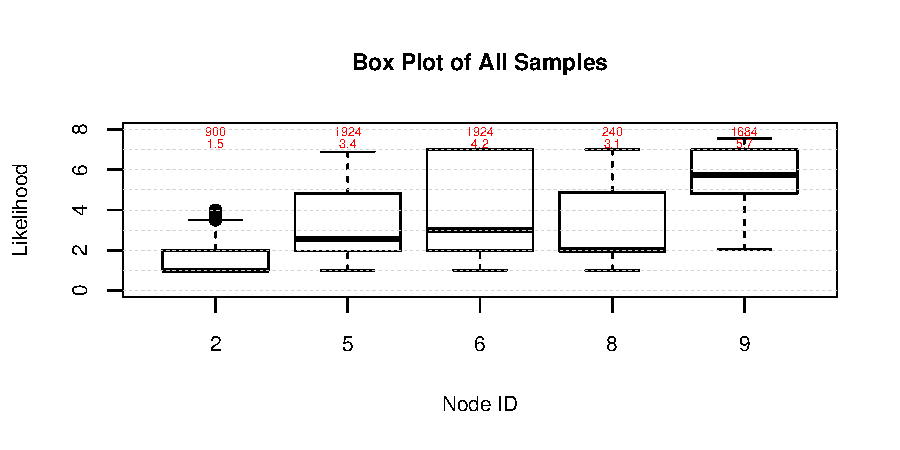
\includegraphics[width=\textwidth]{figs/cart_box1.pdf}
    \caption{\label{fig:cartBox1}}
    \end{subfigure}
    \begin{subfigure}[b]{.48\textwidth}
    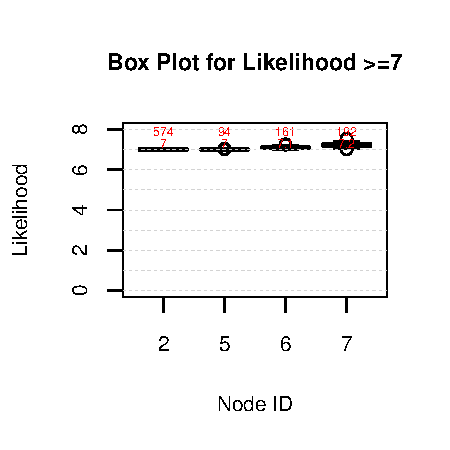
\includegraphics[width=\textwidth]{figs/cart_box2.pdf}
    \caption{\label{fig:cartBox2}}
    \end{subfigure}
    \caption{CART analysis of the parameter space. (i)~Stage~1 where the
        parameter space was sampled coarsely. There are two regimes
    that can be observed which provide better fit.}
\end{figure}
%%
\subsection{Predicting the spread in Southeast Asia}
\label{sec:predict}
We considered three scenarios of introduction of the pest to the region.
The first scenario corresponds to evolution of the spread from Bangladesh
(B1). The other two are hypothetical scenarios based on the analysis in
Section~\ref{sec:entry}. Scenario~M corresponds to \tuta{} introduced near
a major port region of Malaysia. The third Scenario~P is its introduction
to Philippines close to the captial city Manila assuming introduction
due to migratory workers from \tuta{} affected regions.

The spatio-temporal spread for Scenario~B1 is shown in
Figure~\ref{fig:spreadBGD}. The start time corresponds to~24 time steps (or
two years) from the first report. The results indicate that there is a high
chance that \tuta{} will spread to Mainland Southeast Asia in four to six
years. Because of long distance dispersal, we also observe a non-radial
spread. Aided by domestic trade and exports from Thailand, there is
possibility that the pest will be introduced to Peninsular Malaysia and
subsequently to Singapore and Indonesia in this period even though this
area is much farther from the current range of \tuta{}. Also, we see the
possibility of the pest crossing the sea from Peninsular Malaysia to
Malaysian Borneo within a year of introduction to this country. However,
these are conservative estimates. First of all, the simulations do not
account for possible new introductions. Secondly, there are boundary
effects; we have not accounted for cells belonging to Northeastern parts of
India that share border with Bangladesh and Myanmar and the Yunnan province
of China. Both these factors can only aid in the spread.

The spread due to other two scenarios are shown in Figures~\ref{spreadMYS}
and~\ref{spreadPHL} respectively. Note that in both of these scenarios we do not
account for the spread from Bangladesh. This is crucially dependent on the
time of introduction. However, it is critical to consider the synergistic
effects of range expansion from multiple locations. The spread in
Scenario~M follows a similar pattern as in Scenario~B3.
\aacomment{Philippines pending}.

\begin{figure}[ht]
    \centering
    \begin{subfigure}[b]{.32\textwidth}
        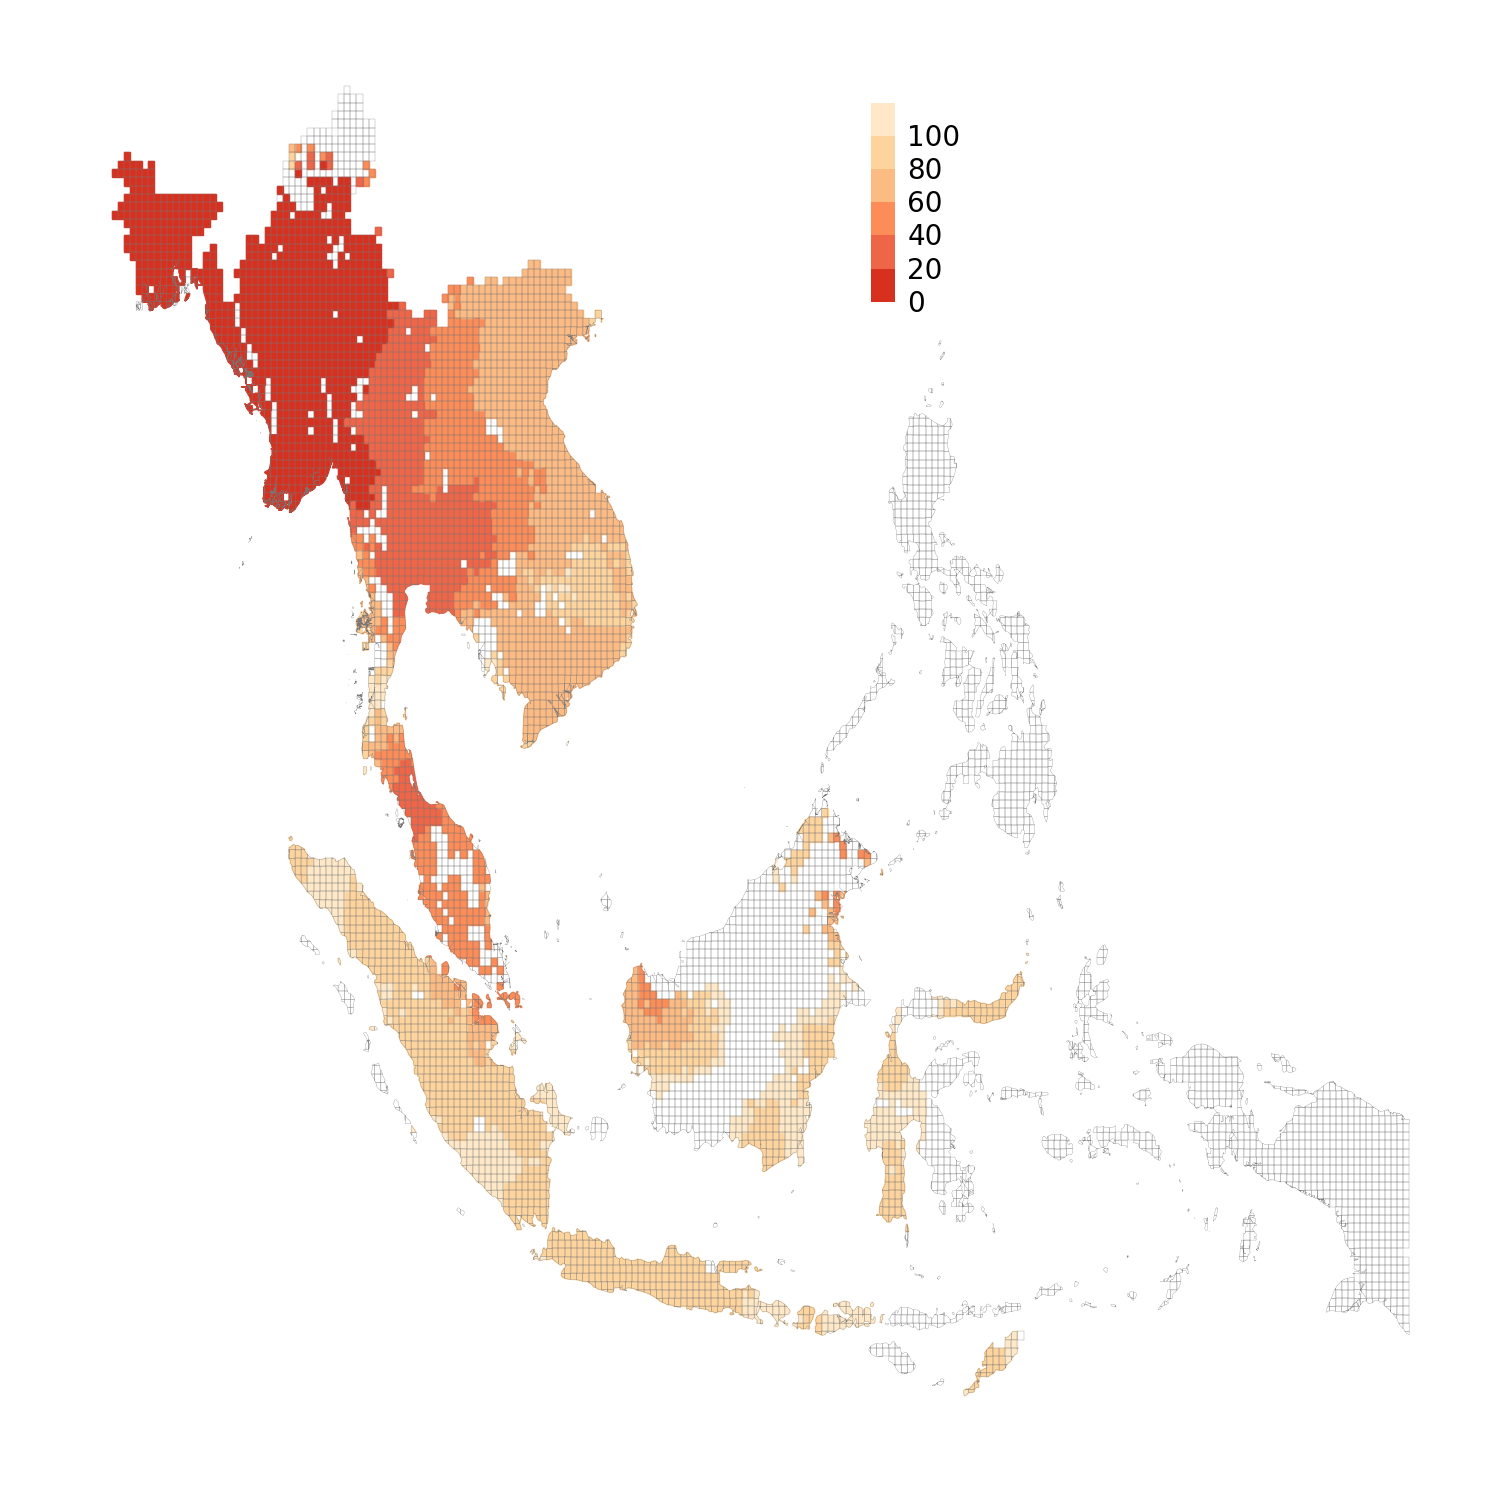
\includegraphics[width=\textwidth,trim={3cm 3cm 8cm 3cm},clip]{figs/spread_BGD.png}
    \caption{Scenario~B1\label{fig:spreadBGD}}
    \end{subfigure}
    \begin{subfigure}[b]{.32\textwidth}
        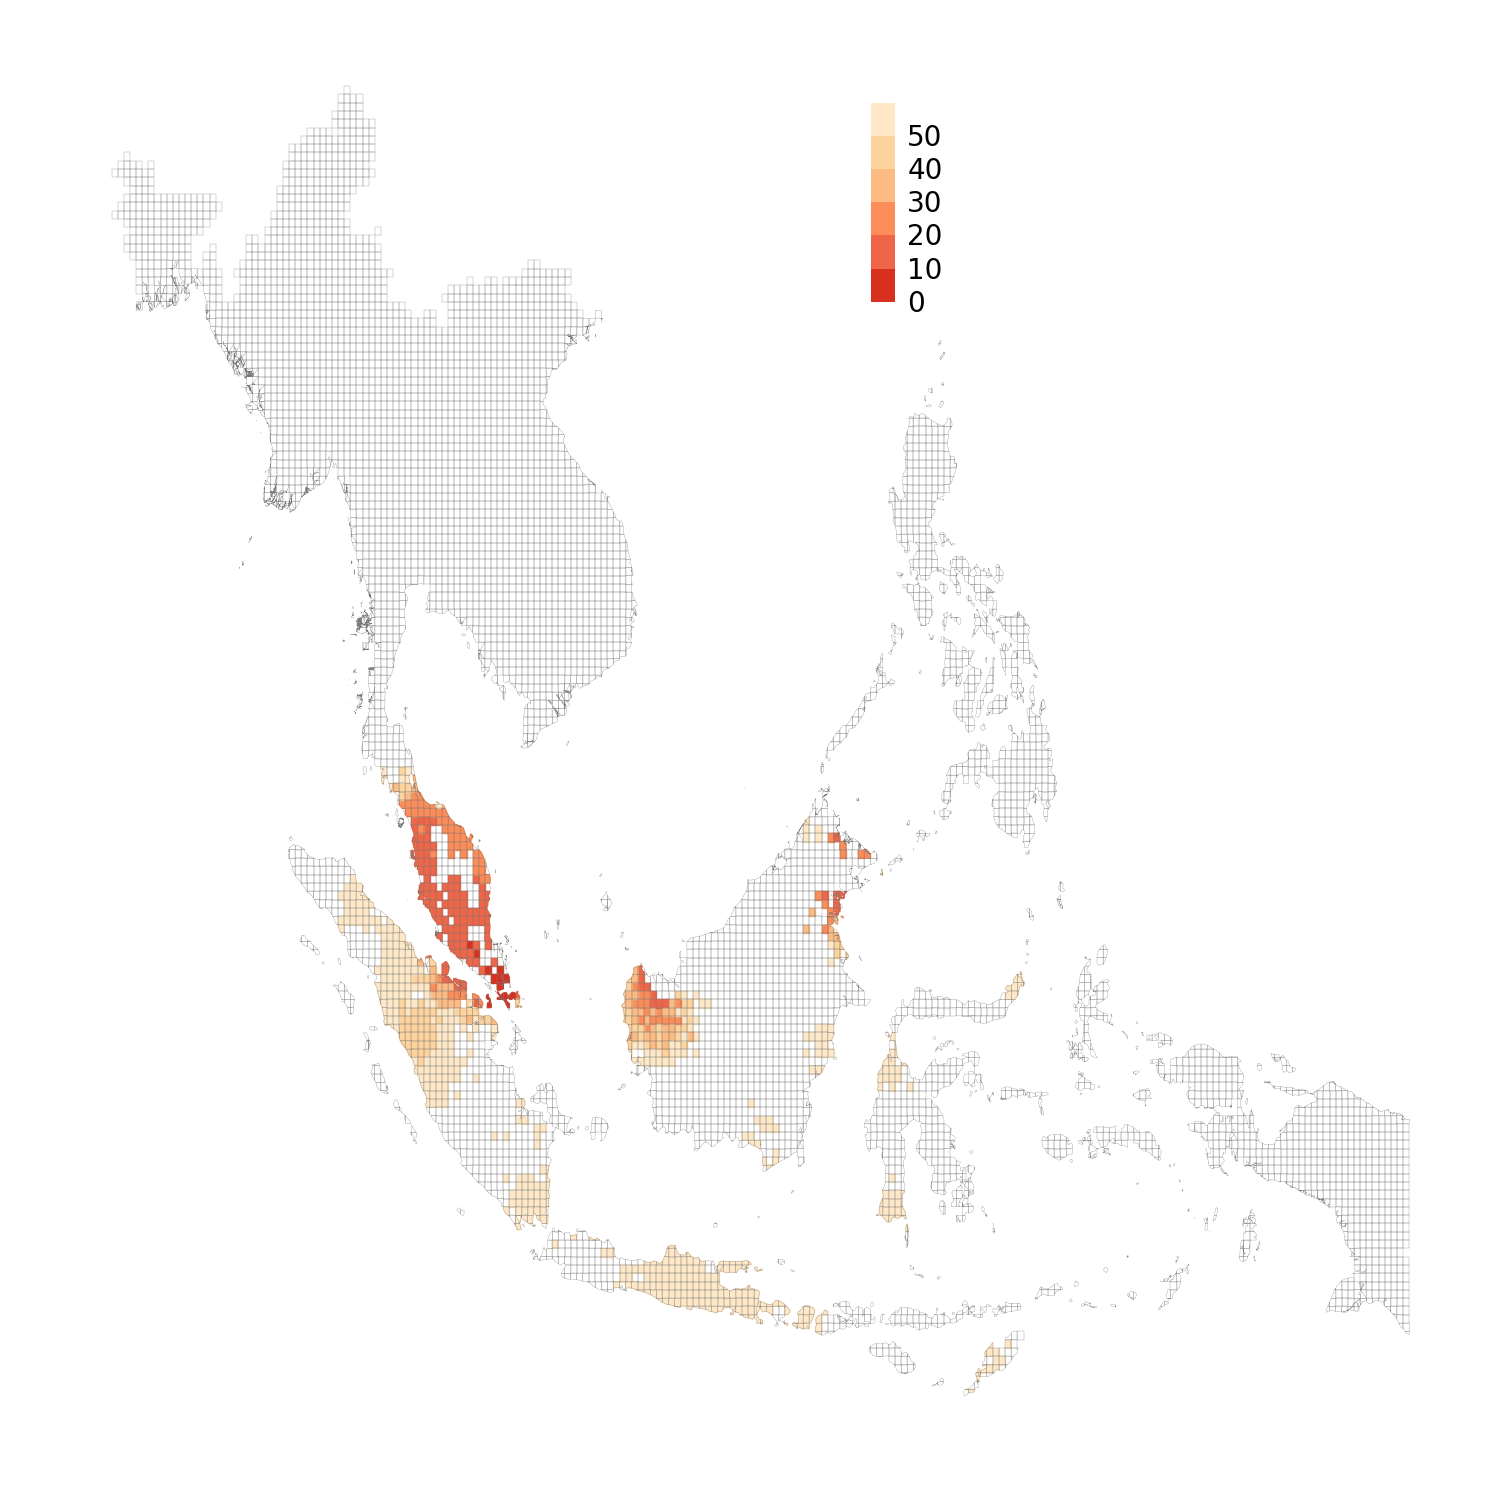
\includegraphics[width=\textwidth,trim={4cm 2cm 8cm 12cm},clip]{figs/spread_MYS.png}
    \caption{Scenario~M\label{fig:spreadMYS}}
    \end{subfigure}
    \begin{subfigure}[b]{.32\textwidth}
        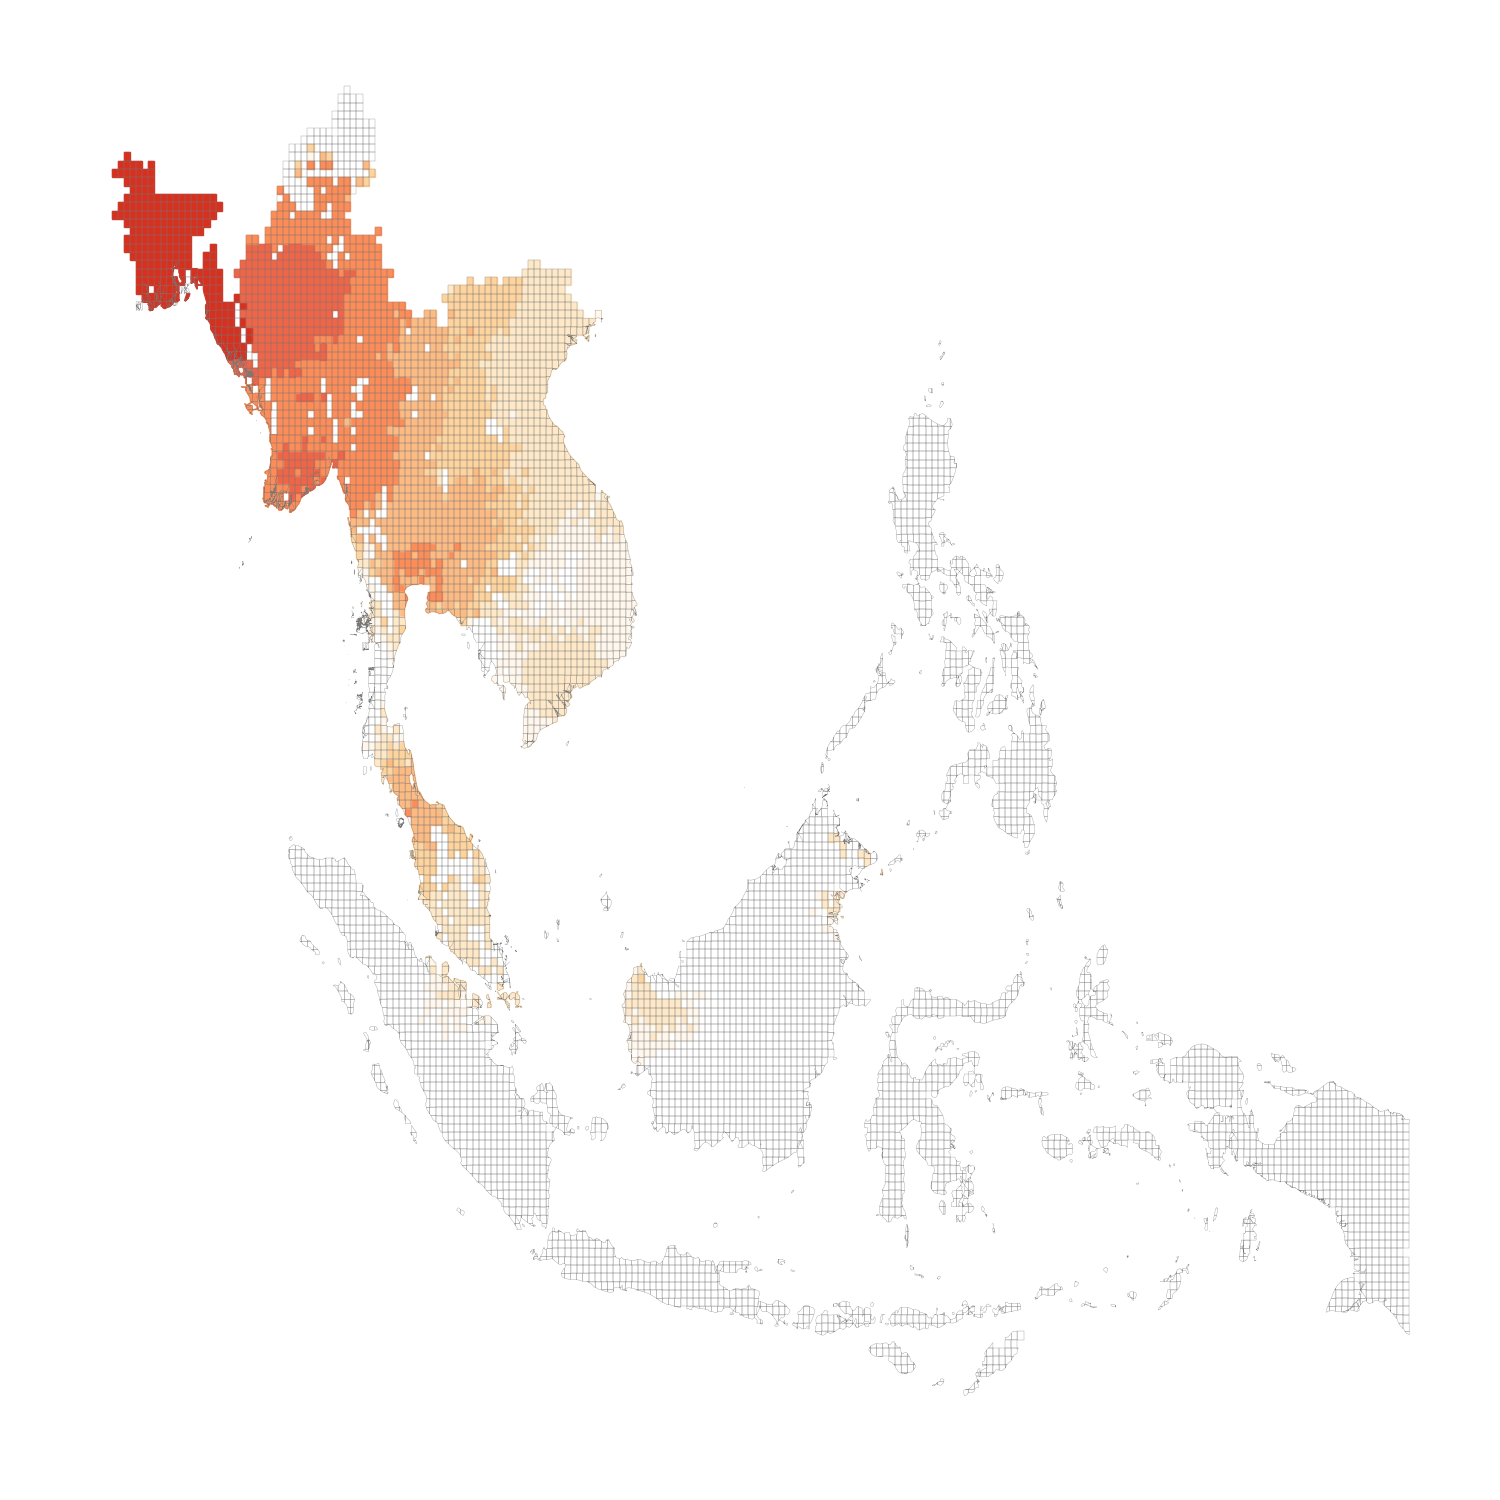
\includegraphics[width=\textwidth,trim={4cm 2cm 8cm 12cm},clip]{figs/spread_PHL.png}
    \caption{Scenario~P\label{fig:spreadPHL}}
    \end{subfigure}
    \caption{Possible spread of \tuta{} in the focus region under three
    scenarios. In each plot, the legends correspond to months. For the
    purpose of plotting, for each cell, we compute the time~$t$ for which
    the empirical probability of infection before~$t$ is at least $0.1$.
    Scenario~B3 starts with Bangladesh and significant parts of Myanmar
    infested accounting for spread from May 2016 to May 2018.
    \aacomment{Philippines pending, legend will be made bigger}}
\end{figure}

%%
%% Specific observations
%% \begin{itemize}
%%     \item identify important vegetable production areas
%% \end{itemize}

%% \subsection{Understanding the role of interventions}
%% Since there is strong indication that trade is a significant pathway for
%% the rapid spread of \tuta{}, it is important to consider methods to reduce
%% the effect of this pathway. An obvious way of accomplishing this is to
%% monitor localities by setting up pheromone traps and taking necessary
%% management steps to mitigate long distance jumps. But it is not practical
%% to implement as it is hard to spread awareness and set up traps in each and
%% every locality, particularly in this region where many countries lack the
%% required infrastructure.  Nopsa~et~al.~\cite{nopsa2015ecological}
%% considered this problem in the context of soybean rust in the US, modeling
%% the spread as a propagation process over a network of counties. They
%% developed efficient strategies to reduce the spread by identifying and
%% monitoring only a subset of locations which are critical for the spread.
%% However, their strategies heavily rely on the history of infections,
%% which is absent in our case.  Here, we evaluate a simple strategy. First,
%% we select a fraction of localities in each country (5\% and 10\%) with high
%% annual outflow. For a locality, this is obtained by aggregating $O_i(t)$
%% for $t=1,2,\ldots,12$. The reasoning for this strategy is as follows.
%% Should such a locality be infected, since it has high outflow it has the
%% potential to influence several of its long distance neighbors, thus aiding
%% in rapid spread of the pest. Under the assumption that appropriate control
%% measures are taken, we reduce the incoming and outgoing edge weights
%% by~$50\%$ of their original value. The resulting model was compared with
%% the case where no action is taken (Section~\ref{sec:predict}).
%% 
%% Farm-level \aacomment{not sure about this}
%% \begin{itemize}
%%     \item suitability threshold is varied
%%     \item Scenario 1 where for all cells it is done
%%     \item Scenario 2 where for it is done in key tomato growing areas
%%     \item Scenario 3 where it is done only near localities
%% \end{itemize}
%% 
%% Market-level
%% \begin{itemize}
%%     \item Scenario 1: we identify localities which are hubs (lots of
%%     outflow) and reduce their flow.
%% \end{itemize}
%% %%
%% \begin{figure}[ht]
%%     \centering
%%     \begin{subfigure}[b]{.47\textwidth}
%%         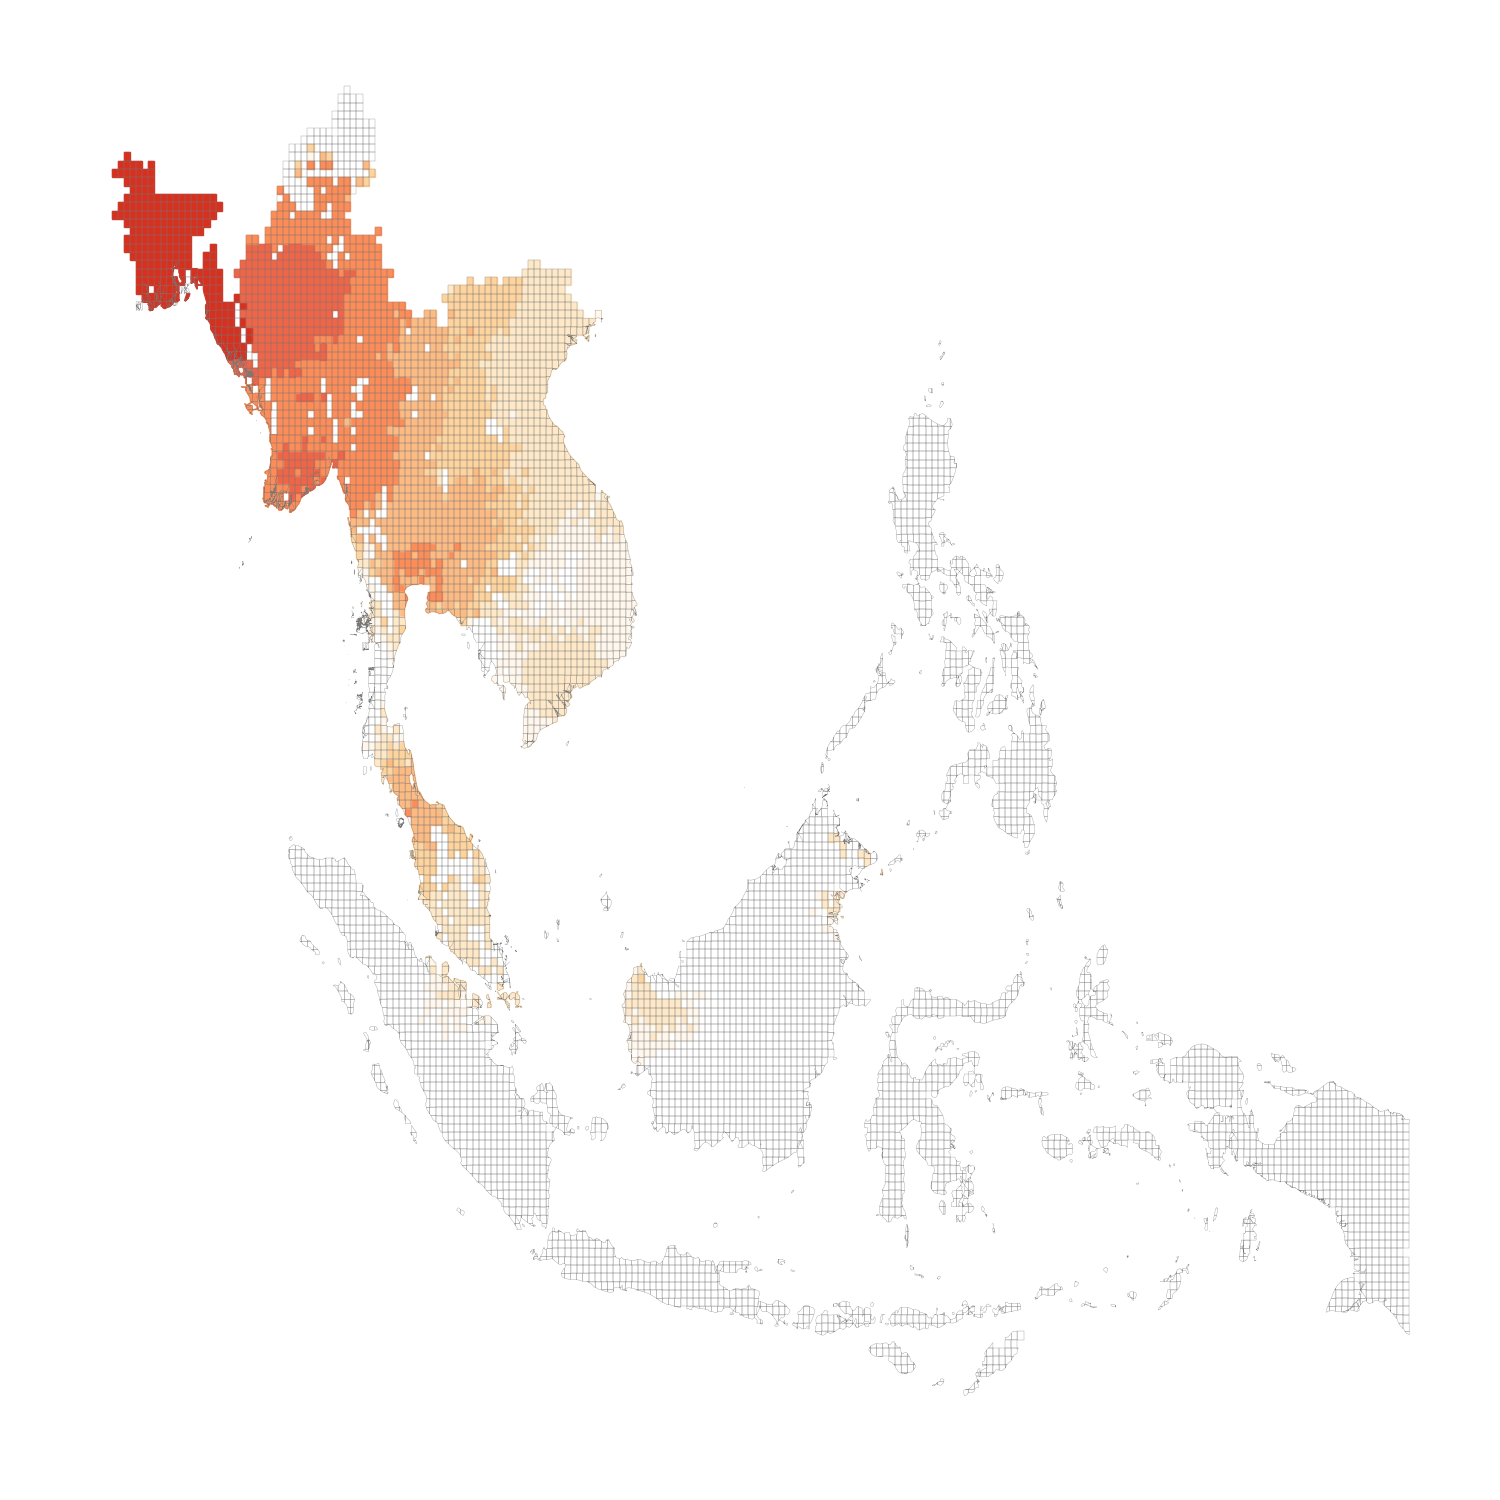
\includegraphics[width=\textwidth]{figs/spread_farm_level_interventions.png}
%%     \caption{\label{fig:spreadFarmLevel}}
%%     \end{subfigure}
%%     \begin{subfigure}[b]{.47\textwidth}
%%     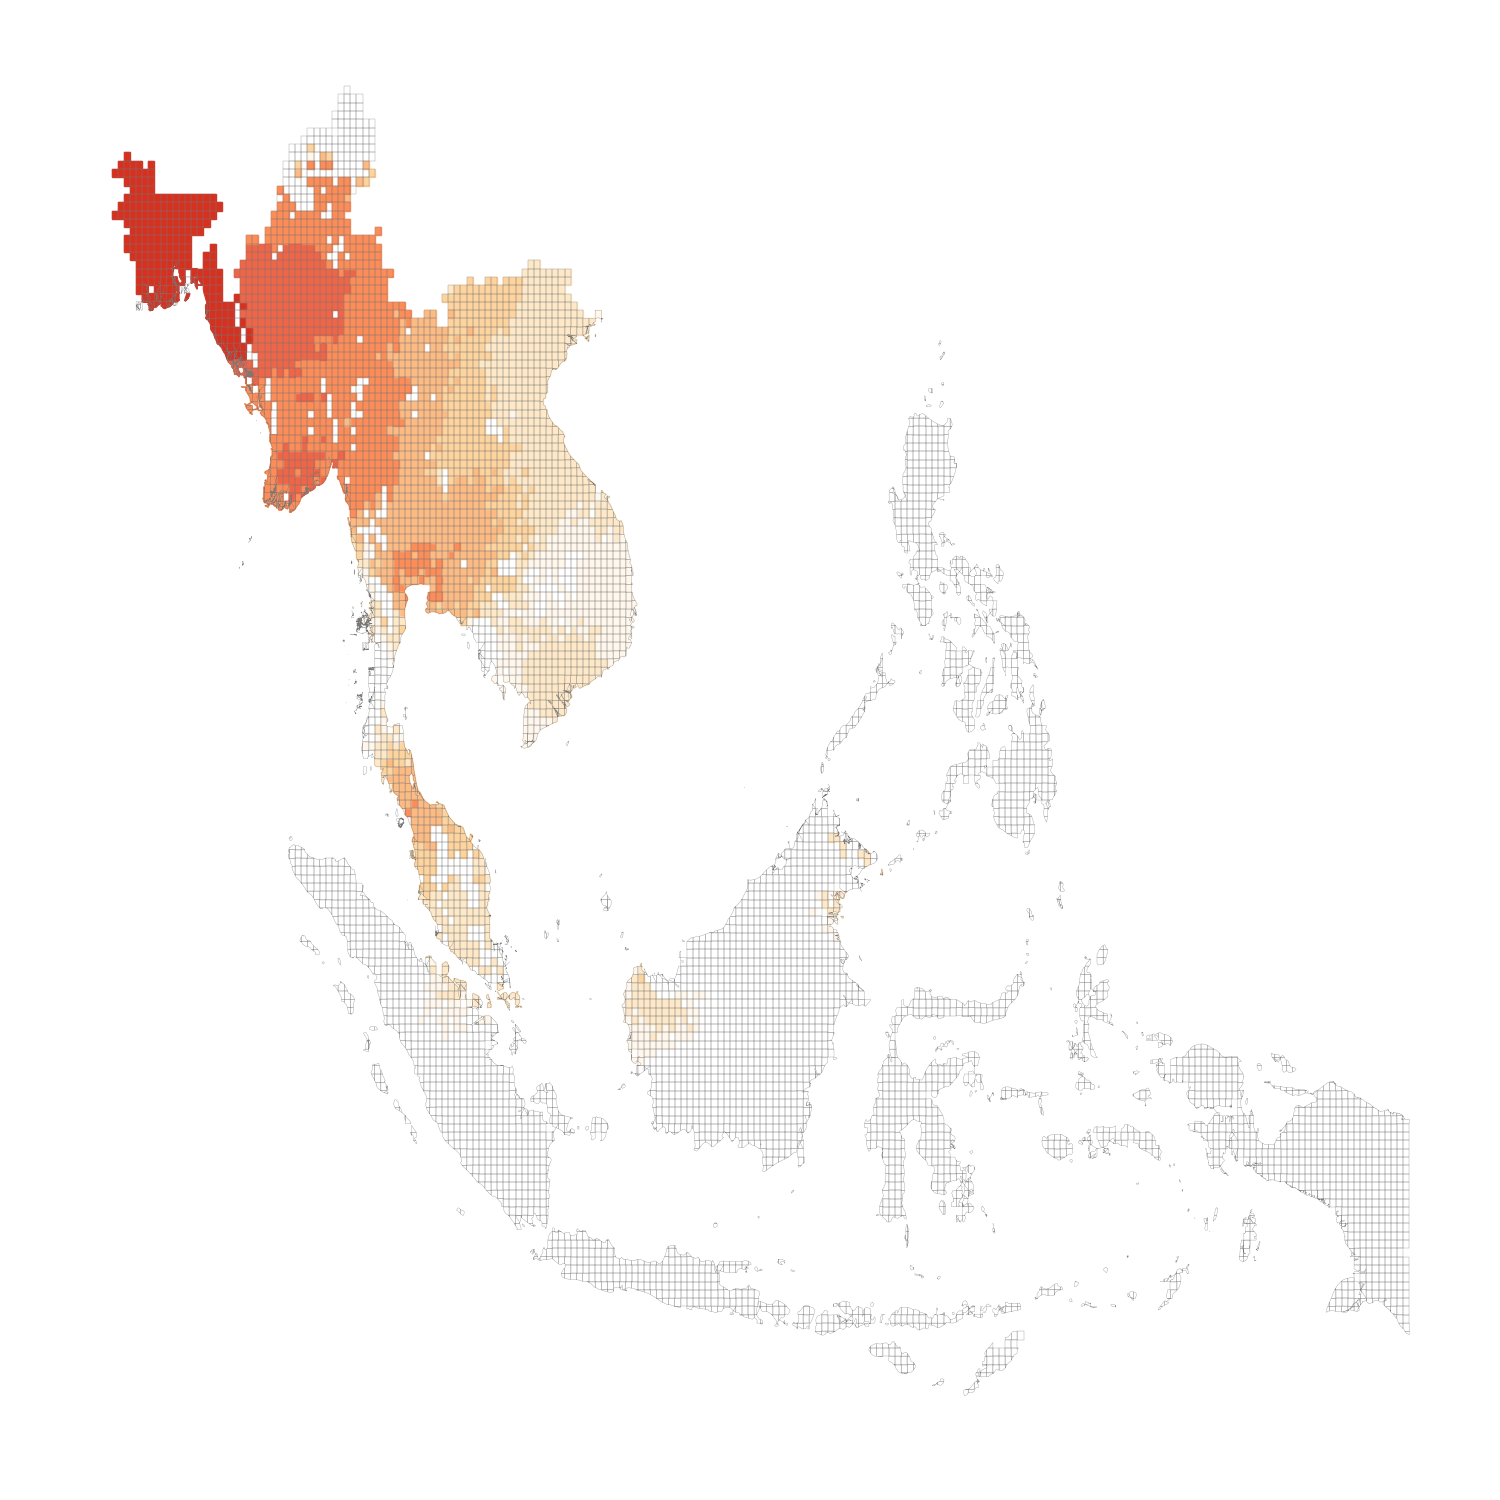
\includegraphics[width=\textwidth]{figs/spread_market_level_interventions.png}
%%     \caption{\label{fig:spreadMarketLevel}}
%%     \end{subfigure}
%%     \caption{Effect of interventions}
%% \end{figure}

\subsection{Sensitivity analysis}
\begin{itemize}
    \item all alphas, start month, initial condition, Moore range, latency
    period
\item CART comes here
\item If we focus on all
instances of parameters for which likelihood is greater than~$12$ ($75\%$
match),
\end{itemize}
%%
\section{Discussion}
This study is very relevant and timely considering that crops such as
tomato, eggplant, and potato are among the top vegetables in most of these
countries.  Traditionally, these crops have been grown in the winter during
the dry season. However, over the past decade, due to rising
demand--domestic as well as from neighboring countries--there has been a
thrust towards year-round production using protected cultivation methods and
resilient varieties~\cite{ali2001,moustier2007}. Also the food industry is gradually
restructuring: supermarkets replacing traditional
food chains. Therefore, invasions from
pests such as \tuta{} can have a huge negative impact on the socioeconomic
fabric of this region. Besides invasive species spread, there are other
applications where understanding production and trade dynamics of major
crops is useful or even essential. These include studies of natural or
human-initiated disasters~\cite{}, climate change, nutrition~\cite{}, etc.

In recent years, there has been a thrust towards integrated modeling
approaches to understand invasive species dynamics. Multi-pathway models
have been analyzed to study the role of human-mediated
dispersal~\cite{robinet2009role,robinet2012human,carrasco2010unveiling}.
Robinet~et~al.~\cite{robinet2009role} show that the distribution and spread
pattern of the pinewood nematode in China is strongly correlated with
density of human population and infrastructure such as railways and river
ports. A similar approach was applied to the pine processionary
moth~\cite{robinet2012human}.  Carrasco~et~al.~\cite{carrasco2010unveiling}
combine spatially explicit models with a phenology model to incorporate
population dynamics of the pest (western corn rootworm). Like the previous
works, this work accounts for human population. Carrasco~et~al. consider two types of
long-distance dispersals -- domestic and international. The domestic mode
is modeled as a flow network between cities using a gravity model approach.
The flow between two cities is a function of human population of these
cities and the distance between them.
Nopsa~et~al.~\cite{nopsa2015ecological} use a network science approach to
studying the role of transport and storage infrastructure in the spread of
pests and pathogens of wheat. Sutrave~et~al.~\cite{sutrave2012identifying}
use a time-varying network model to study the spread of Soybean rust.
However, in all these cases, there was more information available on the
incidence of the pest or pathogen under study enabling validation of the
developed models. For emerging pests, this is nearly impossible to obtain
such incidence reports, particularly
in countries that lack awareness or infrastructure,

Our model is in part motivated by the hybrid approaches used in the study of
infectious diseases of humans and livestock~(for
example~\cite{bradhurst2015hybrid,yang2016}).
Bradhurst~et~al.~\cite{bradhurst2015hybrid} study the spread of foot and
mouth disease in livestock by using an aggregate population-level model to
capture within-herd spread and an individual-based model for between herd
spread. This is much like our approach of capturing local and long-distance
human-mediated spread. A similar approach is used by
Yang~et~al.~\cite{yang2016} to forecast influenza outbreaks. They use a
patch network model where a compartmental model is used to simulate
intra-locale spread and a gravity model based approach is used for
inter-locality spread of flu in the neighborhoods of New~York.

\paragraph{Key challenges.}
We have used a multitude of datasets-- production, consumption, trade
dynamics, climate, biology, etc.-- to capture, to a reasonable extent, the
complexity of the invasion process. A major challenge was data inadequacy.
For many countries such as Vietnam, Cambodia, and Laos, production data had
to be collected (or even inferred) from several publications and
reports~\cite{}. Therefore, data came from disparate sources (multi-type,
different countries, etc.), and were misaligned in time (different years)
and spatial resolution (grid to country level). Production and trade data
from FAOSTAT also had gaps in it.  In particular, it was hard to model
seasonal production and human assisted spread. Seasonal production is
dependent not only on the host, climate, and geography, but also on people's
preferences and market demand. For most countries, only qualitative
information is available. Another example is the modeling of consumption.
It is possible that there is lot of variation in consumption within a
country~\cite{wijk2007} as well as across seasons. Even at the country
level, data is available for only half of the countries. Also, we did not
find any correlation between consumption and GDP or tomato production
(correlation $< 0.01$). To determine outflows and inflows for each locality,
we had to identify major ports for imports and exports as well as estimate
fraction of production which was used for processing. This data was
available only for a couple of countries.

\paragraph{Limitations.}
The fidelity of models such as the one presented here crucially depends on
the availability of quality data as well as a good understanding of the
processes involved. As pointed out on multiple occasions, the
scarcity of data has forced us to greatly simplify some of the processes.
However, the developed framework is modular and extensible. Given
high-resolution accurate datasets and a better knowledge of the processes,
individual modules can be replaced with more sophisticated modeling
approaches.  One example is the use of volume of production of preferred
host crops as a surrogate for population. In the future, complex phenology
models can be used instead to model accurately the growth of the pest under
specific conditions. This would require years of study of the tritrophic
interactions concerning the pest, host, and its indigenous predators (like
for example, the work by Carrasco~et~al.~\cite{carrasco2010unveiling}).
However, as cautioned by Robinet~et~al.~\cite{robinet2012suite}, this would
add to the complexity of the model making it near impossible to verify
and validate.

The farm--market-consumer interactions (local human-mediated spread) are
well understood at a conceptual level. More or less, in all the countries
of the focus region, the structure remains the same. It involves various
actors such as farmers, wholesalers, retailers, wet markets, supermarkets,
etc. Nevertheless, it is nearly impossible to accurately model the dynamics.
Rebaudo~et~al.~\cite{rebaudo2011}, for example, use a complex
agent-based model to study just the interaction between farmers of two
villages in the context of the potato moth in Ecuador. Similarly, given data on
actual flow of vegetables, the gravity model can be improved or replaced by
more sophisticated approaches. The natural spread pathway can be further
improved by taking into account wind trajectories.

Applying this generic modeling approach to other study regions or other
pests would require taking into account additional factors. For example,
seedling trade could be an important pathway, particularly in the European
and the Mediterranean region as well as North America. From a production
perspective, it is becoming important to factor in protected cultivation
methods, which have enabled farmers to extend the growing season. Also, it
is important to study account for damage done by the pest.
 \begin{itemize}
     \item is volume of trade representative?
     \item need to talk about impact to China and Australia.
 \end{itemize}

%%
\section*{Acknowledgments}
This work was supported in part by the United States Agency for
International Development under the Cooperative Agreement NO.
AID-OAA-L-15-00001 Feed the Future Innovation Lab for Integrated Pest
Management, DTRA CNIMS Contract HDTRA1-11-D-0016-0001, NSF BIG DATA Grant
IIS-1633028, NSF DIBBS Grant ACI-1443054, NIH Grant 1R01GM109718 and NSF
NRT-DESE Grant DGE-154362.

We are grateful to Yousuf Mian, Nguyen Van Hoa, and Kim Hian for their help
with obtaining country-specific information on production, trade, and pest
incidence.
\bibliographystyle{plain}
\bibliography{refs}
\end{document}

